\documentclass[a4paper,14pt, unknownkeysallowed]{extreport}

\usepackage{cmap} % Улучшенный поиск русских слов в полученном pdf-файле
\usepackage[T2A]{fontenc} % Поддержка русских букв
\usepackage[utf8]{inputenc} % Кодировка utf8
\usepackage[english,russian]{babel} % Языки: русский, английский
\usepackage{enumitem}


\usepackage{threeparttable}

\usepackage[14pt]{extsizes}

\usepackage{caption}
\captionsetup{labelsep=endash}
\captionsetup[figure]{name={Рисунок}}

% \usepackage{ctable}
% \captionsetup[table]{justification=raggedleft,singlelinecheck=off}

\usepackage{amsmath}

\usepackage{geometry}
\geometry{left=30mm}
\geometry{right=10mm}
\geometry{top=20mm}
\geometry{bottom=20mm}

\usepackage{titlesec}
\titleformat{\section}
	{\normalsize\bfseries}
	{\thesection}
	{1em}{}
\titlespacing*{\chapter}{0pt}{-30pt}{8pt}
\titlespacing*{\section}{\parindent}{*4}{*4}
\titlespacing*{\subsection}{\parindent}{*4}{*4}

\usepackage{setspace}
\onehalfspacing % Полуторный интервал

\frenchspacing
\usepackage{indentfirst} % Красная строка

\usepackage{titlesec}
\titleformat{\chapter}{\LARGE\bfseries}{\thechapter}{20pt}{\LARGE\bfseries}
\titleformat{\section}{\Large\bfseries}{\thesection}{20pt}{\Large\bfseries}

\usepackage{multirow}
\usepackage{listings}
\usepackage{xcolor}

% Для листинга кода:
\lstset{%
	language=python,   					% выбор языка для подсветки	
	basicstyle=\small\sffamily,			% размер и начертание шрифта для подсветки кода
	numbers=left,						% где поставить нумерацию строк (слева\справа)
	numberstyle=\tiny,		     		% размер шрифта для номеров строк
	stepnumber=1,						% размер шага между двумя номерами строк
	numbersep=5pt,						% как далеко отстоят номера строк от подсвечиваемого кода
	frame=single,						% рисовать рамку вокруг кода
	tabsize=4,							% размер табуляции по умолчанию равен 4 пробелам
	captionpos=t,						% позиция заголовка вверху [t] или внизу [b]
	breaklines=true,					
	breakatwhitespace=true,				% переносить строки только если есть пробел
	backgroundcolor=\color{white},
	basicstyle=\footnotesize\ttfamily,
	keywordstyle=\color{blue},
	stringstyle=\color{red},
	commentstyle=\color{gray}
	showspaces=false,
    showstringspaces=false
}


\usepackage{pgfplots}
\usetikzlibrary{datavisualization}
\usetikzlibrary{datavisualization.formats.functions}


\lstset{
	literate=
	{а}{{\selectfont\char224}}1
	{б}{{\selectfont\char225}}1
	{в}{{\selectfont\char226}}1
	{г}{{\selectfont\char227}}1
	{д}{{\selectfont\char228}}1
	{е}{{\selectfont\char229}}1
	{е}{{\"e}}1
	{ж}{{\selectfont\char230}}1
	{з}{{\selectfont\char231}}1
	{и}{{\selectfont\char232}}1
	{й}{{\selectfont\char233}}1
	{к}{{\selectfont\char234}}1
	{л}{{\selectfont\char235}}1
	{м}{{\selectfont\char236}}1
	{н}{{\selectfont\char237}}1
	{о}{{\selectfont\char238}}1
	{п}{{\selectfont\char239}}1
	{р}{{\selectfont\char240}}1
	{с}{{\selectfont\char241}}1
	{т}{{\selectfont\char242}}1
	{у}{{\selectfont\char243}}1
	{ф}{{\selectfont\char244}}1
	{х}{{\selectfont\char245}}1
	{ц}{{\selectfont\char246}}1
	{ч}{{\selectfont\char247}}1
	{ш}{{\selectfont\char248}}1
	{щ}{{\selectfont\char249}}1
	{ъ}{{\selectfont\char250}}1
	{ы}{{\selectfont\char251}}1
	{ь}{{\selectfont\char252}}1
	{э}{{\selectfont\char253}}1
	{ю}{{\selectfont\char254}}1
	{я}{{\selectfont\char255}}1
	{А}{{\selectfont\char192}}1
	{Б}{{\selectfont\char193}}1
	{В}{{\selectfont\char194}}1
	{Г}{{\selectfont\char195}}1
	{Д}{{\selectfont\char196}}1
	{Е}{{\selectfont\char197}}1
	{е}{{\"E}}1
	{Ж}{{\selectfont\char198}}1
	{З}{{\selectfont\char199}}1
	{И}{{\selectfont\char200}}1
	{Й}{{\selectfont\char201}}1
	{К}{{\selectfont\char202}}1
	{Л}{{\selectfont\char203}}1
	{М}{{\selectfont\char204}}1
	{Н}{{\selectfont\char205}}1
	{О}{{\selectfont\char206}}1
	{П}{{\selectfont\char207}}1
	{Р}{{\selectfont\char208}}1
	{С}{{\selectfont\char209}}1
	{Т}{{\selectfont\char210}}1
	{У}{{\selectfont\char211}}1
	{Ф}{{\selectfont\char212}}1
	{Х}{{\selectfont\char213}}1
	{Ц}{{\selectfont\char214}}1
	{Ч}{{\selectfont\char215}}1
	{Ш}{{\selectfont\char216}}1
	{Щ}{{\selectfont\char217}}1
	{Ъ}{{\selectfont\char218}}1
	{Ы}{{\selectfont\char219}}1
	{Ь}{{\selectfont\char220}}1
	{Э}{{\selectfont\char221}}1
	{Ю}{{\selectfont\char222}}1
	{Я}{{\selectfont\char223}}1
}

\usepackage{graphicx}
\newcommand{\img}[3] {
	\begin{figure}[h!]
		\center{\includegraphics[height=#1]{img/#2}}
		\caption{#3}
		\label{img:#2}
	\end{figure}
}


\usepackage[justification=centering]{caption} % Настройка подписей float объектов

\usepackage[unicode,pdftex]{hyperref} % Ссылки в pdf
\hypersetup{hidelinks}

\usepackage{csvsimple}

\newcommand{\code}[1]{\texttt{#1}}

\usepackage{longtable}

\usepackage{array}
\usepackage{booktabs}
\usepackage{floatrow}

\floatsetup[longtable]{LTcapwidth=table}

\def\UrlBreaks{\do\/\do-\do\_}

\makeatletter
\renewcommand*\l@chapter[2]{%
  \ifnum \c@tocdepth >\m@ne
    \addpenalty{-\@highpenalty}%
    \vskip 1.0em \@plus\p@
    \setlength\@tempdima{1.5em}%
    \begingroup
      \parindent \z@ \rightskip \@pnumwidth
      \parfillskip -\@pnumwidth
      \leavevmode \bfseries
      \advance\leftskip\@tempdima
      \hskip -\leftskip
      #1\nobreak\normalfont\leaders\hbox{$\m@th
        \mkern \@dotsep mu\hbox{.}\mkern \@dotsep
        mu$}\hfill\nobreak\hb@xt@\@pnumwidth{\hss #2}\par
      \penalty\@highpenalty
    \endgroup
  \fi}
\makeatother

\begin{document}



\setcounter{page}{4}
\renewcommand{\contentsname}{Содержание} 
\tableofcontents


\setcounter{page}{5}
\chapter*{Введение}
\addcontentsline{toc}{chapter}{Введение}

В настоящие время компьютерное графическое моделированию различных предметов приобрело большую популярность, многие компании стали к нему прибегать, чтобы избавиться от недопонимания между заказчиком и исполнителем. Такой подход дает возможность как можно четче обозначить детали проекта, и реже допускать ситуации, в которых становится известно, что исполнитель неправильно воспринял идею заказчика. Мною была выбрана тема, связанная с визуализацией трехмерного городского пространства. Данная программа может быть использована при планировке городских дворов.

Для исполнителя важно исключить возникновение правок на поздних стадиях выполнения работы. Поэтому важно предоставить реалистичное изображение на этапе предварительного показа. Для построения такого изображения, которое позволит понять пользователю концепцию работы, потребуется учитывать невидимость ребер объектов сцены по отношению к наблюдателю и освещение отдельных участков рабочей плоскости.

\textbf{Целью} курсовой работы является реализация программного обеспечения для трехмерного планировщика городского пространства.

Для достижения поставленной цели необходимо выполнить следующие задачи.

\begin{itemize}
	\item Описать список доступных к размещению на сцене моделей, формализовать эти модели.
	\item Выбрать существующие алгоритмы компьютерной графики для визуализации сцены и объектов на ней.
	\item Выбрать язык программирования и среду разработки.
	\item Реализовать выбранные алгоритмы визуализации.
	\item Реализовать программное обеспечения для визуализации и редактирования городского пространства.
\end{itemize}





\chapter{Аналитическая часть}

\section[Описание и формализация объектов сцены]{Описание и формализация объектов\linebreak сцены}

Сцена состоит из следующих объектов.

\begin{itemize}
	\item \textbf{Площадка сцены} -- правильный параллелепипед с заданной сеткой, по которой расставляются модели. Объекты располагаются только на одной из сторон площадки. Размеры границ задаются количеством ячеек (квадратов) по ширине и длине площадки. Размер ячеек -- константная величина, определяемая внутри программы. Пользователь может вращать сцену с объектами. Цвет площадки -- салатовый.
	\item \textbf{Объекты сцены}  -- модели, расположенные на площадке сцены, которые занимают определенное количество клеток сетки (ячеек). Каждая модель представляет собой набор граней, описываемых точками в пространстве, которые соединены ребрами. Все доступные модели определены заранее, в программе не предусмотрена возможность добавления новых или изменения старых моделей. В ПО доступна возможность изменения положения или удаления объектов на сцене.
	
	Список доступных объектов сцены.
	\begin{enumerate}
		\item \textbf{Дом.} Состоит из трех частей: стен, крыши и окон. 
		
		\begin{itemize}
			\item Стена дома представляет собой плоскость, перпендикулярную плоскости сцены. Длиной и шириной стены является заданное пользователем число ячеек (квадратов) на сетке сцены. По середине каждого квадрата стены оставлено квадратное отверстие для окна дома, площадь которого равна $\frac{1}{9}$ площади ячейки сцены. Высота дома задается пользователем (кол-во ячеек сцены). Высота одного этажа равна длине ячейки (квадрата) сетки сцены. Цвет стены -- оранжевый.
			\item Крыша дома состоит из четырех плоскостей: двух треугольных и двух четырехугольных, имеющих формы равнобедренных трапеций. Нижнии вершины этих трапеций совпадают с вершинами углов стен верхнего этажа дома. Высота крыши дома соответствует длине ячейки сетки сцены. Цвет крыши -- красный.
			\item Окно дома представляют собой квадратную плоскость, перпендикулярную плоскости сцены. Площадь окна равна $\frac{1}{9}$ площади ячейки сетки сцены. Окна расставляются в оставленных при построение стен пустотах. Цвет окна -- желтый.
		\end{itemize}

		\item \textbf{Машина.} Занимает одну клетку сетки сцены по ширине и две клетки по длине. Представляется набором плоскостей, образующими в отдельности кузов машины, ее колеса и стекла. Основой кузова является параллелепипед, расположенный на высоте $\frac{1}{6}$ длины клетки над плоскостью сцены. Длина и высота колеса машины соответствуют $\frac{1}{4}$ длины ячейки сетки сцены. Машина может быть расположена как вдоль оси $X$, так и вдоль оси $Y$.  Цвет кузова машины -- фиолетовый, колес -- серый, окон -- белый.


		\item \textbf{Дорога.} Представляет собой квадратную плоскость, параллельную плоскости сцены. Занимает одну клетку по ширине и длине. Состоит из двух частей: асфальта и полосы. Ширина полосы соответствует $\frac{1}{5}$ длины ячейки сетки сцены, а длина -- $\frac{3}{4}$ длины ячейки. Дорога может быть расположена как вдоль оси $X$, так и вдоль оси $Y$. Цвет асфальта -- серый, полосы -- белый.
		
		\item \textbf{Дерево.} Занимает одну клетку по ширине, длине и две по высоте. Состоит из двух частей: ствола и листвы.
		
		\begin{itemize}
			\item Ствол дерева представляет собой параллелепипед, высотой одна клетка, ширина и высота которого соответствуют $\frac{1}{5}$ длины ячейки сетки сцены.
			\item Листва дерева состоит из набора параллелепипедов, которые вместе занимают одну клетку по ширине, длине и высоте. Цвет листвы -- зеленый.
		\end{itemize}

	\end{enumerate}	
	
	Деревья, дома, дороги разрешено расставлять только на свободных клетках сетки сцены, машины -- только на дорогах. Дороги не должны прилегать к дому.
	
	\item \textbf{Источник света} -- материальная точка пространства. Принимает ортогональную проекцию визуализируемой сцены из своего положения с некоторым ограниченным обзором. В зависимости от расположения источника и направления распространения лучей света, определяется тень от объектов, расположенных на сцене. Положение источника света задается относительно текущей точки наблюдения последовательными поворотами по осям X и Y.
\end{itemize}


\section{Выбор способа определения моделей на сетке сцены}

Использование моделей позволяет правильно отображать форму и размеры объектов сцены. 

Модели могут задаваться в следующих формах.

\begin{itemize}
	\item \textbf{Каркасная модель.} В данной модели задается информация о вершинах и ребрах объекта. Это одна из простейших форм задания модели. Основная проблема отображения объектов с помощью каркасной модели заключается в том, что модель не всегда однозначно передает представление о форме объекта.
	\item \textbf{Поверхностная модель.} Данный тип модели часто используется в компьютерной графике. Поверхность может описываться аналитически, либо задаваться другим способом. Недостатком поверхностной модели является отсутствие информации о том, с какой стороны поверхности находится материал.
	\item \textbf{Твердотельная модель.} Данная форма задания модели отличается от поверхностной формы тем, что в объемных моделях к информации о поверхностях добавляется информация о том, с какой стороны расположен материал. Это можно сделать путем указания направления внутренней нормали.
\end{itemize}

Для решения поставленной задачи не подойдет каркасная форма модели, так как такое представление будет приводить к неправильному восприятию заказчиком форм объекта. Твердотельная модель также не подойдет, так как пользователю совершенно не важно, из какого материала будет выполнен тот или иной объект сцены. Поэтому выбираем поверхностную форму модели.

\section[Выбор способа задания поверхностных моделей]{Выбор способа задания поверхностных\linebreak моделей}

Существует несколько способов задать поверхностную модель.

\begin{itemize}
	\item \textbf{Аналитический способ.} Этот способ задания модели характеризуется описанием модели объекта, которое доступно в неявной форме, то есть для получения визуальных характеристик необходимо дополнительно вычислять некоторую функцию, которая зависит от параметра.
	\item \textbf{Полигональная сетка.} Данный способ характеризуется совокупностью вершин, ребер и граней, определяющих форму объекта в трехмерном пространстве.
\end{itemize}

Рассмотрим существующие способы хранения информации о сетке.

\begin{itemize}
	\item \textbf{Cписок граней.} Объект -- это множество граней и множество вершин. В каждую грань входят как минимум 3 вершины.
	\item \textbf{<<Крылатое>> представление.} Каждая точка ребра указывает на две вершины, две грани и четыре ребра, которые ее касаются.
	\item \textbf{Полуреберные сетки.} То же <<крылатое>> представление, но информация обхода хранится для половины грани.
	\item \textbf{Таблица углов.} Таблица, хранящая вершины. Обход заданной таблицы неявно задает полигоны. Такое представление более компактно и более производительно для нахождения полигонов, но, в связи с тем, что вершины присутствуют в описании нескольких углов, операции по их изменению медленны.
	\item \textbf{Вершинное представление.} Хранятся лишь вершины, которые указывают на другие вершины. Простота представления дает возможность проводить над сеткой множество операций.
\end{itemize}

При выборе способа задания модели в курсовом проекте решающим фактором стала скорость выполнения преобразований над объектами сцены.

Оптимальное для реализации представление - модель, заданная полигональной сеткой. Такая модель позволит избежать проблем при описании сложных объектов сцены.

Способом хранения полигональной сетки был выбран список граней, так как это даст явное описание граней. Этот способ позволит эффективно преобразовывать модели, так как структура будет включать в себя список вершин.


\section[Выбор алгоритма удаления невидимых ребер и поверхностей]{Выбор алгоритма удаления невидимых\linebreak ребер и поверхностей}

Задача удаления невидимых линий и поверхностей является одной из наиболее сложных в машинной графике. Алгоритмы удаления невидимых линий и поверхностей служат для определения линий ребер, поверхностей или объемов, которые видимы или невидимы для наблюдателя, находящегося в заданной точке пространства. Решать поставленную задачу удаления можно как в объектном пространстве (в мировой системе координат), так и в пространстве изображения (в экранных координатах).

Свойства, которыми должен обладать алгоритм, для оптимальной работы реализуемого программного обеспечения:

\begin{itemize}
	\item алгоритм должен быть достаточно быстрым при работе с множеством объектов сцены, чтобы пользователь не ожидал долгой загрузки изображения;
	\item алгоритм может работать в любом пространстве (скорость важнее точности).
\end{itemize}

Рассмотрим алгоритмы для удаления невидимых ребер и поверхностей.

\subsection{Алгоритм Робертса}

Данный алгоритм работает в объектном пространстве, решая задачу только с выпуклыми телами.

Алгоритм выполняется в 3 этапа.

\begin{enumerate}
	\item \textbf{Этап подготовки исходных данных.} 
	
	На данном этапе должна быть задана информация о телах. Для каждого тела сцены должна быть сформирована матрица тела $V$. Размерность матрицы -- $4 * n$, где $n$ -- количество граней тела.
	
	Каждый столбец матрицы представляет собой четыре коэффициента уравнения плоскости $ax + by + cz + d = 0$, проходящей через очередную грань.

	Таким образом, матрица тела будет представлена в следующем виде:

	\begin{equation}
		V = \begin{pmatrix}
			a_{1} & a_{2} & \ldots & a_{n}\\
			b_{1} & b_{2} & \ldots & b_{n}\\
			c_{1} & c_{2} & \ldots & c_{n}\\
			d_{1} & d_{2} & \ldots & d_{n}
		\end{pmatrix}
	\end{equation}

	Матрица тела должна быть сформирована корректно, то есть любая точка, расположенная внутри тела, должна располагаться по положительную сторону от каждой грани тела. В случае, если для очередной грани условие не выполняется, соответствующий столбец матрицы надо умножить на $-1$. Для проведения проверки следует взять точку, расположенную внутри тела. Координаты такой точки можно получить путем усреднения координат всех вершин тела.

	\item \textbf{Этап удаления ребер, экранируемых самим телом.} 
	
	На данном этапе рассматривается вектор взгляда $E = \{0, 0, -1, 0\}$.
	Для определения невидимых граней достаточно умножить вектор $E$ на матрицу тела $V$. Отрицательные компоненты полученного вектора будут соответствовать невидимым граням.

	\item \textbf{Этап удаления невидимых ребер, экранируемых другими телами сцены.}
	
	На данном этапе для определения невидимых точек ребра требуется построить луч, соединяющий точку наблюдения с точкой на ребре. Точка будет невидимой, если луч на своем пути встречает в качестве преграды рассматриваемое тело. Если тело является преградой, то луч должен пройти через тело. Если луч проходит через тело, то он находится по положительную сторону от каждой грани тела.
\end{enumerate}

\subsubsection{Преимущества и недостатки алгоритма Робертса}

\textbf{Преимущества:}

\begin{itemize}
	\item алгоритм работает в объектном пространстве, точность вычислений высокая.
\end{itemize}

\textbf{Недостатки:}

\begin{itemize}
	\item теоретический рост сложности алгоритма -- квадрат числа объектов. Для решения данной проблемы достаточно воспользоваться модифицированными реализациями, например, с использованием габаритных тестов или сортировки по оси z;
	\item все тела сцены должны быть выпуклыми. Данная проблема также приводит к усложнению алгоритма, так как потребуется прибегнуть к проверке объектов на выпуклость и их разбиению на выпуклые многоугольники.
\end{itemize}

\subsubsection{Вывод}

Алгоритм Робертса не подходит для решения поставленной задачи по следующим причинам:

\begin{itemize}
	\item от программного обеспечения не требуется той точности визуализации объектов, которую предоставляет алгоритм;
	\item на сцене может находиться множество объектов, что замедлит скорость работы алгоритма. Это не удовлетворяет преподнесенным требованиям к скорости выполнения алгоритма. Особенные проблемы также могут наблюдаться при наличии множества невыпуклых тел на сцене;
	\item реализация модификаций, позволяющих приблизить рост сложности алгоритма к линейной, очень труднозатратна.
\end{itemize}

\subsection{Алгоритм, использующий z-буфер}

Данный алгоритм работает в пространстве изображения. Используется два буфера:
\begin{itemize}
	\item буфер кадра, в котором хранятся атрибуты каждого пикселя в пространстве изображения;
	\item z-буфер, куда помещается информация о координате $z$ для каждого пикселя.
\end{itemize}

Первоначально в z-буфере находятся минимально возможные значения z, а в буфере кадра располагаются пиксели, описывающие фон. Каждый многоугольник преобразуется в растровую форму и записывается в буфер кадра.

В процессе подсчета глубины нового пикселя, он сравнивается с тем значением, которое уже лежит в z-буфере. Если новый пиксель расположен ближе к наблюдателю, чем предыдущий, то он заносится в буфер кадра и происходит корректировка z-буфера.

Для решения задачи вычисления глубины $z$ каждый многоугольник описывается уравнением $ax + by + cz + d = 0$. При $c = 0$ многоугольник для наблюдателя вырождается в линию. 

Для некоторой сканирующей строки $y = const$, поэтому имеется возможность рекуррентно высчитывать $z^\prime$ для каждого $x^\prime = x + dx$:

\begin{equation}
	z^\prime - z = -\frac{ax^\prime + d}{c} +\frac{ax + d}{c} = \frac{a(x - x^\prime)}{c}
\end{equation}

Получим: $z^\prime = z - \frac{a}{c^\prime}$, так как $x - x^\prime = dx = 1$.

При этом стоит отметить, что для невыпуклых многогранников предварительно потребуется удалить нелицевые грани.

\subsubsection{Преимущества и недостатки алгоритма, использующего z-буфер}

\textbf{Преимущества:}

\begin{itemize}
	\item простота реализации;
	\item оценка вычислительной трудоемкости алгоритма линейна;
	\item экономия вычислительного времени, так как элементы сцены не сортируются.
\end{itemize}

\textbf{Недостатки:}

\begin{itemize}
	\item большой объем требуемой памяти;
	\item реализация эффектов прозрачности сложна.
\end{itemize}

\subsubsection{Вывод}

Алгоритм отвечает главному требованию -- скорости работы с множеством объектов. Также простота алгоритма позволит достаточно быстро реализовать данный алгоритм и, что важнее, в полной мере отладить его.

При этом следует отметить, что само изображение будет относительно малых размеров, что приведет к некритично большим затратам памяти для выполнения данного алгоритма.

\subsection{Алгоритм обратной трассировки лучей}

Наблюдатель видит объект посредством испускаемого источником света, который падает на этот объект и согласно законам оптики некоторым путем доходит до глаза наблюдателя. Отслеживать пути лучей от источника к наблюдателю неэффективно с точки зрения вычислений, поэтому наилучшим способом будет отслеживание путей в обратном направлении, то есть от наблюдателя к объекту.

Предполагается, что сцена уже преобразована в пространство изображения, а точка, в которой находится наблюдатель, находится в бесконечности на положительной полуоси $z$, и поэтому световые лучи параллельны этой же оси. При этом каждый луч проходит через центр пикселя растра до сцены. Траектория каждого луча отслеживается для определения факта пересечения определенных объектов сцены с этими лучами. При этом необходимо проверить пересечение каждого объекта сцены с каждым лучом, а пересечение с $z_{min}$ представляет видимую поверхность для данного пикселя.

Если же точка наблюдателя находится не в бесконечности, то есть в рассмотрении фигурирует перспективная проекция, то предполагается, что сам наблюдатель по-прежнему находится на положительной полуоси $z$, а сам растр при этом перпендикуляром оси $z$. Задача будет состоять в том, чтобы построить одноточечную центральную проекцию на картинную плоскость.

Определения пересечений происходит с помощью погружения объектов в некоторую выпуклую оболочку -- например, сферическую. Поиск пересечения с такой оболочкой происходит проще: достаточно проверить превосходит ли радиус сферы-оболочки расстояние от центра этой сферы до луча.

Предположим, что некоторая прямая проходит через две точки $P_1 (x_1, y_1, z_1)$  и $P_2 (x_2, y_2, z_2)$:
\begin{equation}
	P(t) = P_1 + (P_2 - P_1)t
\end{equation}

Компоненты при этом:
\begin{equation}
	x = x_1 + (x_2 - x_1)t = x_1 + at
\end{equation}
\begin{equation}
	y = y_1 + bt
\end{equation}
\begin{equation}
	z = z_1 + ct
\end{equation}

Таким образом минимальное расстояние от этой прямой до некоторой точки $P_0 (x_0, y_0, z_0)$:
\begin{equation}
	d^2 = (x - x_0)^2 + (y - y_0)^2 + (z - z_0)^2
\end{equation}
Где параметр t, который определяет ближайшую точку $P(t)$:

\begin{equation}
	t = - \frac{a(x_1 - x_0) + b(y_1 - y_0) + c(z_1 - z_0)}{a^2 + b^2 + c^2}
\end{equation}

Если $d^2 > R^2$, где $R$ -- радиус сферической оболочки, то луч не может пересечься с объектом.

\subsubsection[Преимущества и недостатки алгоритма обратной трассировки лучей]{Преимущества и недостатки алгоритма обратной трассировки\linebreak лучей}

\textbf{Преимущества:}

\begin{itemize}
	\item высокая реалистичность синтезируемого изображения;
	\item работа с поверхностями в математической форме;
\end{itemize}

\textbf{Недостатки:}

\begin{itemize}
	\item производительность.
\end{itemize}

\subsubsection{Вывод}

Алгоритм не отвечает главному требованию -- скорости работы. Также от реализуемого продукта не требуется высокой реалистичности синтезируемого изображения и возможности работы с поверхностями, заданными в математической форме. Указанные факты говорят о том, что обратная трассировка лучей не подходит для решения поставленной задачи.

Таким образом, в качестве алгоритма удаления невидимых ребер и поверхностей был выбран алгоритм с использованием z-буфера.

\section{Выбор алгоритма построения теней}

При использовании алгоритма обратной трассировки лучей, рассмотренного ранее, построение теней происходит по ходу выполнения алгоритма: пиксел будет затемнен, если испускаемый луч попадает на объект, но не попадает в источник света. Данный алгоритм не подходит для решения поставленной задачи, так как при проведении анализа алгоритмов удаления невидимых ребер он не был выбран в качестве реализуемого.

В качестве алгоритма удаления невидимых линий и поверхностей в предыдущем подпункте был выбран алгоритм с использованием z-буфера, поэтому одним из наилучших вариантов будет модификация указанного метода путем добавления вычисления теневого z-буфера из точки наблюдения, совпадающей с источником света.

Такой подход позволит не усложнять структуру программы, а также избежать проблем адаптации двух различных методов друг к другу, а, следовательно, уменьшить время отладки алгоритма.


\section{Вывод}

Были рассмотрены способы задания трехмерных моделей и выбрана поверхностная форма задания моделей. Также были рассмотрены алгоритмы удаления невидимых ребер: 

\begin{itemize}
	\item алгоритм, использующий z-буфер;
	\item алгоритм Робертса;
	\item алгоритм обратной трассировки лучей.
\end{itemize}

В качестве реализуемого был выбран алгоритм z-буфера, отвечающего двум требованиям: быстрая работа с множеством объектов сцены и преобладание скорости над точностью. Были рассмотрены алгоритмы построения теней. В качестве реализуемого был выбран алгоритм, использующий теневые карты, в работе которого будет использоваться z-буфер.

\chapter{Конструкторская часть}

\section{Требования к программному обеспечению}

Программа должна выполнять следующие функции:

\begin{itemize}
	\item создание сцены с заданным размером;
	\item поворот, перемещение и масштабирование визуализируемой сцены;
	\item добавление, перемещение и удаление объектов сцены;
	\item добавление и удаление источников света на сцене.
\end{itemize}

\section{Общий алгоритм решения поставленной задачи}

\begin{itemize}
	\item Задать размеры сцены, на которой будут размещаться объекты.
	\item Разместить объекты сцены и источники света.
	\item Основываясь на текущем положении наблюдателя, с помощью модифицированного алгоритма, использующего z-буфер, определить падающие от объектов сцены тени и визуализировать обстановку.
\end{itemize}

\section{Алгоритм, использующий z-буфер}

\begin{itemize}
	\item Всем элементам буфера кадра присвоить фоновое значение.
	\item Инициализировать z-буфер минимальным значением глубины.
	\item Для каждого многоугольника сцены в произвольном порядке:
	
	\begin{itemize}
		\item для каждого пикселя, который принадлежит многоугольнику вычислить его глубину $z(x, y)$;
		\item cравнить вычисленную глубину пикселя со значением, которое находится в z-буфере. Если $z(x,y) > z_{buf} (x,y)$, то $z_{buf} (x,y) = z(x,y)$ и $colour(x,y) = specColour$.
	\end{itemize}

	\item Вывести итоговое изображение.
\end{itemize}

На рисунке \ref{fig:alg1} изображена схема алгоритма z-буфера.

\begin{figure}[h]
	\centering
	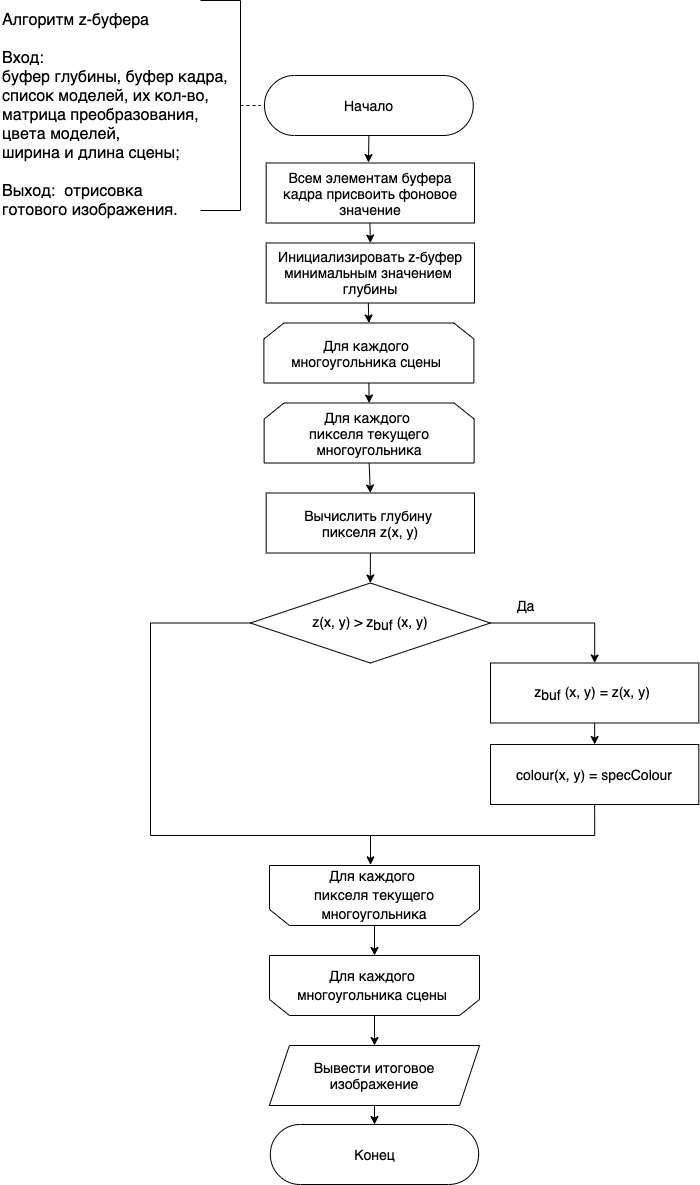
\includegraphics[scale=0.45]{img/scheme_3.png}
	\caption{алгоритм z-буфера}
	\label{fig:alg1}
\end{figure} 


\section[Модифицированный алгоритм, использующий z-буфер]{Модифицированный алгоритм,\linebreak использующий z-буфер}


\begin{itemize}
	\item Для каждого направленного источника света:
	
	\begin{itemize}
		\item инициализировать теневой z-буфер минимальным значением глубины;
		\item определить теневой z-буфер для источника.
	\end{itemize}

	\item Выполнить алгоритм z-буфера для точки наблюдения. При этом, если некоторая поверхность оказалась видимой относительно текущей точки наблюдения, то проверить, видима ли данная точка со стороны источников света.
	
	Для каждого источника света:
	\begin{itemize}
		\item координаты рассматриваемой точки $(x, y, z)$ линейно преобразовать из вида наблюдателя в координаты $(x^\prime, y^\prime, z^\prime)$ на виде из рассматриваемого источника света;
		\item cравнить значение $z_{shadowBuf} (x^\prime, y^\prime)$ со значением $z^\prime(x^\prime, y^\prime)$. Если\linebreak $z^\prime(x^\prime, y^\prime) < z_{shadowBuf} (x^\prime, y^\prime)$, то пиксел высвечивается с учетом его затемнения, иначе точка высвечивается без затемнения.
	\end{itemize}
\end{itemize}

На рисунке \ref{fig:alg2} изображена схема модифицированного алгоритма z-буфера.

\begin{figure}[h]
	\centering
	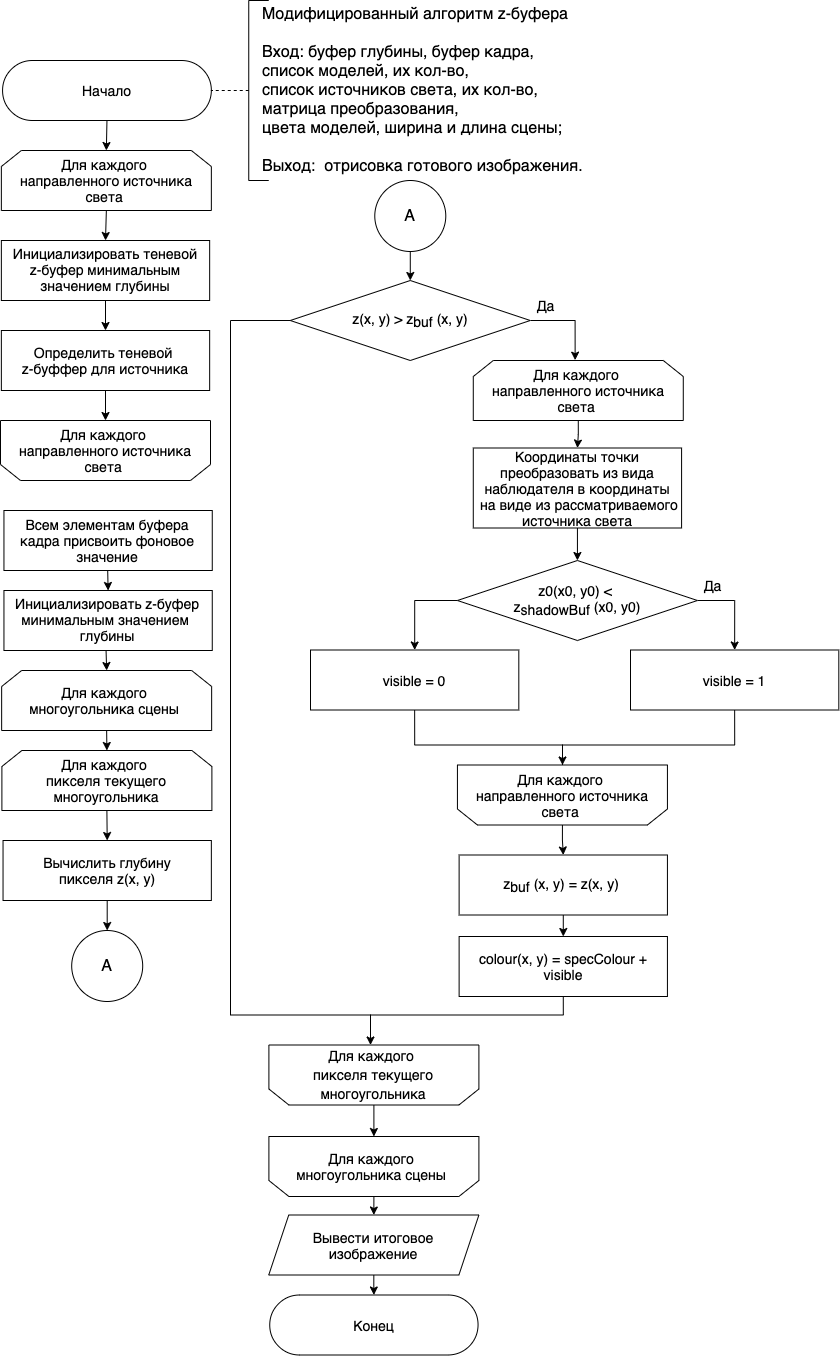
\includegraphics[scale=0.5]{img/scheme_4.png}
	\caption{модифицированный алгоритма z-буфера}
	\label{fig:alg2}
\end{figure} 

\clearpage

\section{Представление данных в ПО}

В таблице \ref{tbl:table_1} описано представление данных в программном обеспечении.

\begin{center}
\captionsetup{justification=raggedright,singlelinecheck=off}
\begin{longtable}[c]{|l|l|}
\caption{Представление данных в ПО\label{tbl:table_1}}
	\\ \hline
	\textbf{Данные} & \textbf{Представление} 
	\\ \hline
	Точка трехмерного пространства & Координаты по осям $x, y, z$
	\\ \hline
	Полигон & Три точки трехмерного пространства
	\\ \hline
	Объект сцены & Список полигонов
	\\ \hline
	Источник света & Угол по осям X и Y относительно \\ & текущей точки наблюдения
	\\ \hline
\end{longtable}
\end{center}

\section{Вывод}

На основе теоретических данных, полученных из аналитического раздела, были описаны требования к програмному обеспечению, общий алгоритм решения задачи, алгоритм z-буфера и модифицированный алгоритм z-буфера, а также было обобщено представление данных в программном обеспечении.


\chapter{Технологическая часть}

\section{Выбор языка программирования и среды разработки}

При написании программного продукта был выбран язык C++. Это обусловлено следующими факторами.

\begin{itemize}
	\item C++ обладает высокой вычислительной производительностью, что очень важно для выполнения поставленной задачи.
	\item Данный язык поддерживает объектно-ориентированную парадигму программирования. Благодаря чему можно приводить объекты сцены к объектам классов, а также пользоваться шаблонами проектирования. Это дает возможность эффективного написания код.
	\item Данный язык преподавался в рамках курса Объектно-Ориентированного Программирования.
	\item Доступность. Для С++ существует большое количество учебной литературы.
\end{itemize}

При написании программы будет задействована среда разработки QT Creator. Данный выбор обусловлен следующими факторами.

\begin{itemize}
	\item Основы работы с данной средой разработки изучались в рамках курса Программирования на Си.
	\item QT Creator позволяет работать с расширением Qt Design, которое позволит создать удобный и надежный интерфейс для программного продукта в сжатые сроки.
\end{itemize}

\clearpage

\section{Структура реализуемых классов}

На рисунках \ref{fig:scheme_1} - \ref{fig:scheme_2} представлена структура реализуемых классов.

\begin{figure}[h]
	\centering
	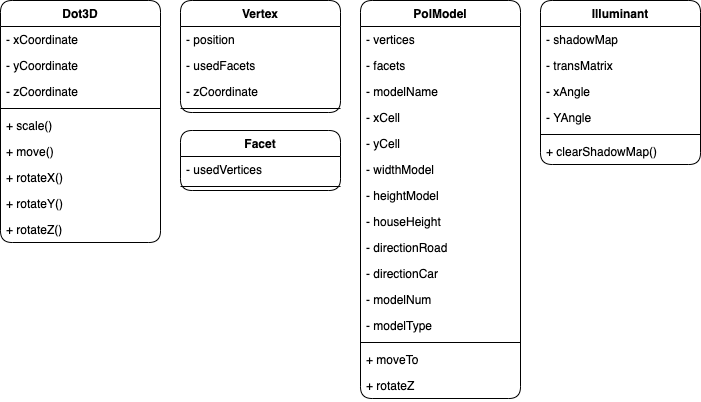
\includegraphics[scale=0.6]{img/scheme_1.png}
	\caption{Структура классов Dot3D, Vertex, Facet, PolModel, Illuminant}
	\label{fig:scheme_1}
\end{figure} 

\begin{itemize}
	\item \textbf{Dot3D} -- класс точки трехмерного пространства. Хранит координаты в
	пространстве, владеет методами преобразований точки.
	\item \textbf{Vertex} -- класс вершины. Хранит координаты точки вершины и номера граней, в которых она задействована.
	\item \textbf{Facet} -- класс грани. Хранит номера задействованных в грани вершин.
	\item \textbf{PolModel} -- класс полигональной модели. Хранит множество вершин и граней, образующих модель, ее имя и координаты ячейки, размеры модели и ось, вдоль которой она расположена. Владеет методами перемещения и вращения по оси Z модели.
	\item \textbf{Illuminant} -- класс источника света. Хранит теневую карту источника, матрицу преобразований и соответствующие ей углы для перемещения текущей точки обзора в точку размещения источника. Владеет методом очистки собственной теневой карты.
\end{itemize}

\clearpage

\begin{figure}[h]
	\centering
	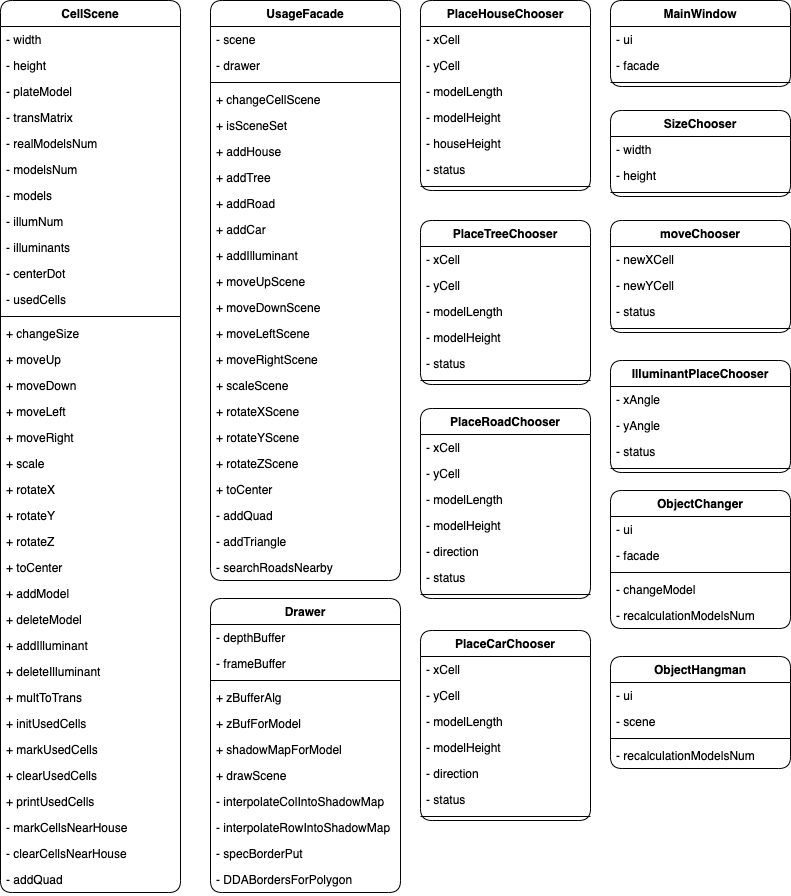
\includegraphics[scale=0.6]{img/scheme_2.png}
	\caption{Структура классов CellScene, Drawer, UsageFacade, PlaceHouseChooser, PlaceTreeChooser, PlaceRoadChooser, PlaceCarChooser, MainWindow, sizeChooser, moveChooser, illuminantPlaceChooser, ObjectChanger, ObjectHangman}
	\label{fig:scheme_2}
\end{figure} 

\clearpage

\begin{itemize}
	\item \textbf{CellScene} -- класс рабочей области сцены. Хранит длину и ширину сцены, модель сцены, на которой размещаются другие объекты, матрицу преобразований для перехода в текущую точку наблюдения, множество моделей интерьера и источников света, размещенных на сцене, и их кол-во, а также точку центра выполнения преобразований. Еще в этом классе хранится матрица использованных клеток сцены. Владеет методами выполнения преобразований над сценой, построения области размещения моделей, добавления и удаления объектов и источников света, отмечания и отчищения занятых клеток в матрице использованных клеток сцены.
	\item \textbf{UsageFacade} -- класс, отвечающий за взаимодействие пользователя с программным обеспечением. Хранит формируемую сцену и класс, отвечающий за растеризацию сцены (наложение сетки, каждая из ячеек которой обрабатывается особым образом). Владеет методами добавления моделей на сцену и преобразований сцены.
	\item \textbf{Drawer} -- класс, отвечающий за растеризацию сцены. Хранит буфер кадра и буфер глубины. Владеет методами алгоритма теневого z-буфера и формирования объекта для отображения рисунка в главном приложении.
	\item \textbf{PlaceHouseChooser} -- класс, связанный с интерфейсом выбора расположения дома (выбора начальной точки модели, ее длины, ширины и высоты).
	\item \textbf{PlaceTreeChooser} -- класс, связанный с интерфейсом выбора расположения дерева (выбора начальной точки модели).
	\item \textbf{PlaceRoadChooser} -- класс, связанный с интерфейсом выбора расположения дороги (выбора начальной точки модели, а также ее ориентации в пространстве).
 	\item \textbf{PlaceCarChooser} -- класс, связанный с интерфейсом выбора расположения машины (выбора начальной точки модели, а также ее ориентации в пространстве).
	\item \textbf{MainWindow} -- точка входа в программу.
	\item \textbf{SizeChooser} -- класс, связанный с интерфейсов выбора размера сцены. Хранит в себе значений длины и ширины создаваемой сцены.
	\item \textbf{moveChooser} -- класс, связанный с интерфейсом выбора нового расположения модели (выбора новой начальной точки модели).
	\item \textbf{IlluminantPlaceChooser} -- класс, связанный с интерфейсом выбора расположения добавляемого источника света. Хранит углы поворота относительно осей X и Y для перехода из точки наблюдения в точку расположения источника света.
	\item \textbf{ObjectChanger} -- класс, связанный с интерфейсом перемещения объектов по сцене. Хранит фасад, с которым в данный момент работает. Владеет методом изменения модели и методом пересчёта номеров моделей на сцене.
	\item \textbf{ObjectHangman} -- класс, связанный с интерфейсом удаления объектов со сцены. Хранит сцену, с которой в данный момент работает. Владеет методом пересчёта номеров моделей на сцене.
\end{itemize}


\section{Сведения о модулях программы}

\begin{itemize}
	\item \textbf{main.cpp} -- главная точка входа в приложение;
	\item \textbf{mainwindow.cpp, mainwindow.h} -- описание и реализация главного окна приложения;
	\item \textbf{mainwindow.ui} -- форма пользовательского интерфейса главного окна приложения;
	\item \textbf{placechooser.cpp, placechooser.hpp} -- описание и реализация классов выбора расположения моделей ($PlaceHouseChooser$, $PlaceTreeChooser$, $PlaceRoadChooser$, $PlaceCarChooser$);
	\item \textbf{placehousechooser.ui} -- форма пользовательского интерфейса класс\linebreak $PlaceHouseChooser$;
	\item \textbf{placetreechooser.ui} -- форма пользовательского интерфейса класса\linebreak $PlaceTreeChooser$;
	\item \textbf{placeroadсhooser.ui} -- форма пользовательского интерфейса класса\linebreak $PlaceRoadChooser$;
	\item \textbf{placecarсhooser.ui} -- форма пользовательского интерфейса класса\linebreak $PlaceCarChooser$;
	\item \textbf{sizechooser.cpp, sizechooser.hpp} -- описание и реализация класса\linebreak $SizeChooser$;
	\item \textbf{sizechooser.ui} -- форма пользовательского интерфейса класса\linebreak $SizeChooser$;
	\item \textbf{illuminantplacechooser.cpp, illuminantplacechooser.hpp} -- описание и реализация класса $IlluminantPlaceChooser$;
	\item \textbf{illuminantplacechooser.ui} -- форма пользовательского интерфейса класса $IlluminantPlaceChoooser$;
	\item \textbf{movechooser.cpp, movechooser.hpp} -- описание и реализация класса\linebreak $moveChooser$;
	\item \textbf{movechooser.ui} -- форма пользовательского интерфейса класса\linebreak $moveChooser$;
	\item \textbf{objectchanger.cpp, objectchanger.hpp} -- описание и реализация класса $objectChanger$;
	\item \textbf{objectchanger.ui} -- форма пользовательского интерфейса класса\linebreak $objectChanger$;
	\item \textbf{objecthangman.cpp, objecthangman.hpp} -- описание и реализация класса $objectHangman$;
	\item \textbf{objecthangman.ui} -- форма пользовательского интерфейса класса\linebreak $objectHangman$;
	\item \textbf{additivemathelements.cpp, additivemathelements.hpp} -- описание и реализация классов математических объектов;
	\item \textbf{objects.cpp, objects.hpp} -- описание и реализация класса полигональных моделей, источников света и сцены.
	\item \textbf{usagefacade.cpp, usagefacade.hpp} -- описание и реализация классов $UsageFacade$ и $Drawer$;
\end{itemize}

\section{Интерфейс программного обеспечения}

На рисунке \ref{fig:interface} изображен интерфейс главного окна программного обеспечения.

\begin{figure}[h]
	\centering
	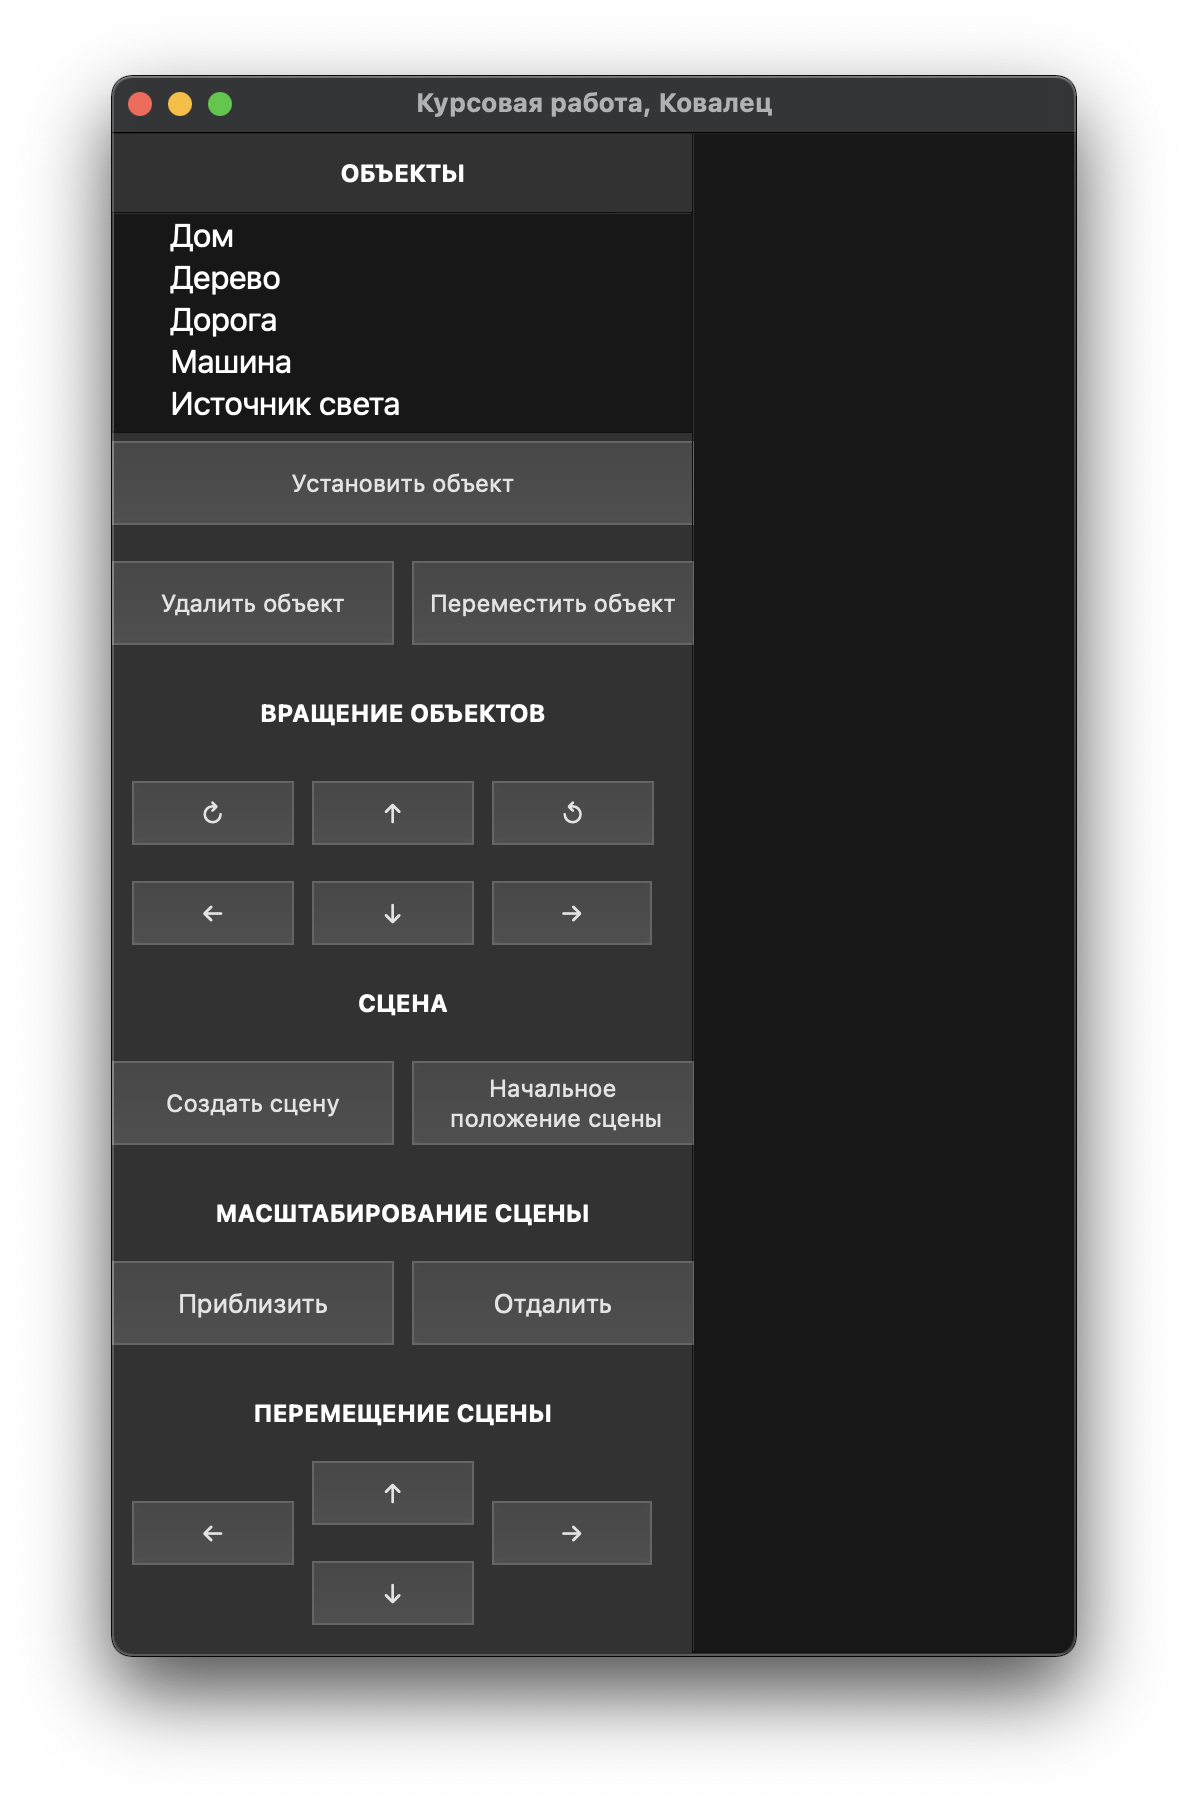
\includegraphics[scale=0.5]{img/interface.png}
	\caption{Интерфейс главного окна ПО}
	\label{fig:interface}
\end{figure} 

Интерфейс главного окна ПО позволяет: 
\begin{itemize}
	\item создавать сцену с объектами, масштабировать ее и перемещать в центр преобразования;
	\item расставлять объекты на клетки сетки сцены, перемещать и удалять их, а также вращать объекты вместе с сценой.
\end{itemize}

На рисунке \ref{fig:scene} изображен интерфейс окна выбора размеров новой сцены. 

\begin{figure}[h]
	\centering
	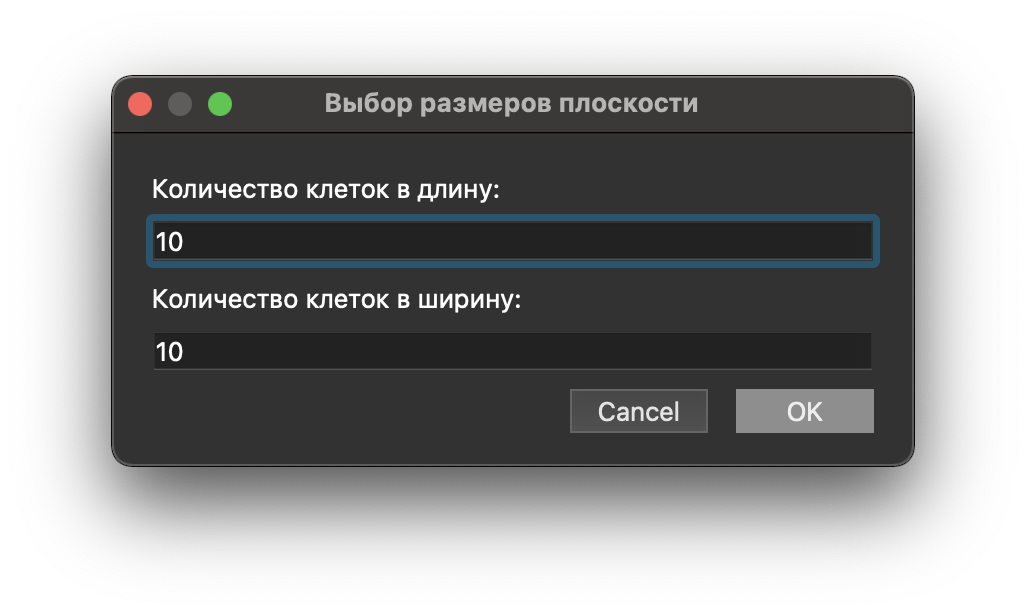
\includegraphics[scale=0.55]{img/scene.png}
	\caption{Интерфейс окна выбора размеров новой сцены}
	\label{fig:scene}
\end{figure} 

На рисунках \ref{fig:house} - \ref{fig:car} изображены интерфейсы окон выбора размеров новых объектов. 

\begin{figure}[h]
	\centering
	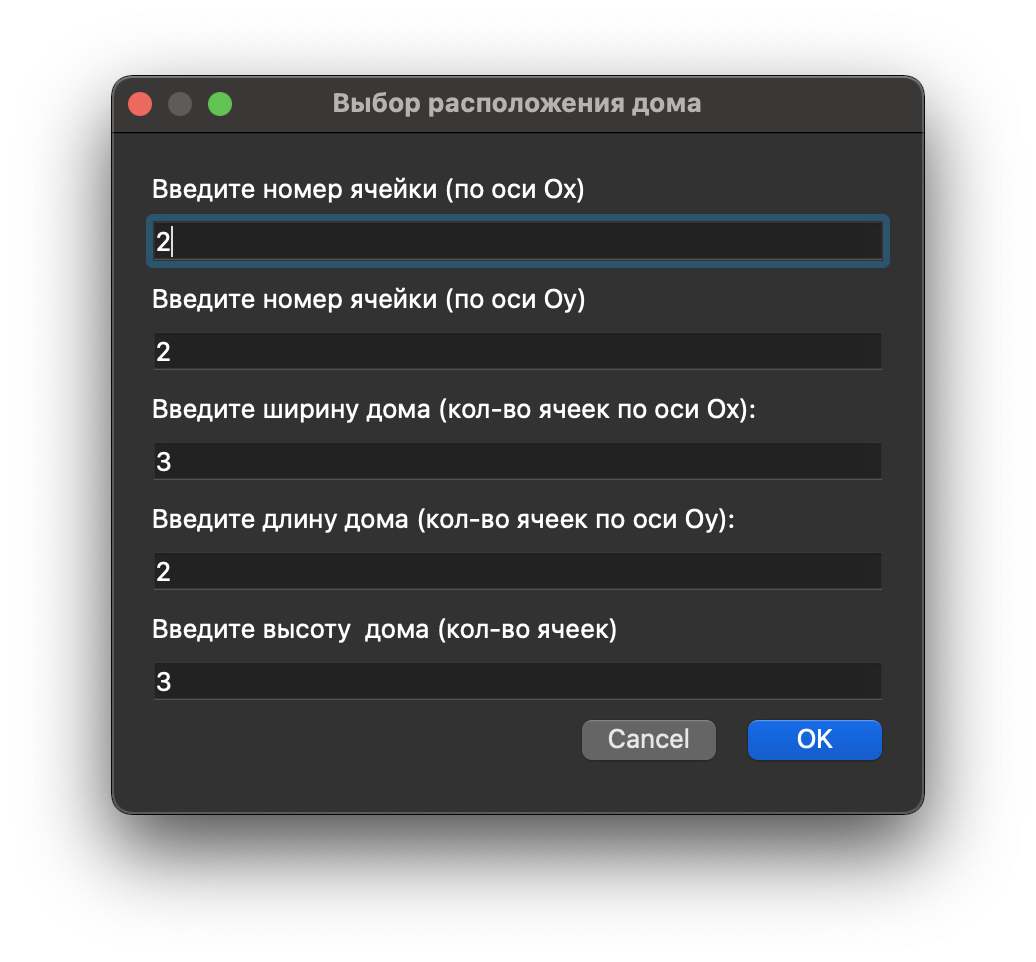
\includegraphics[scale=0.55]{img/house.png}
	\caption{Интерфейс окна выбора распоожения дома}
	\label{fig:house}
\end{figure} 

\begin{figure}[h]
	\centering
	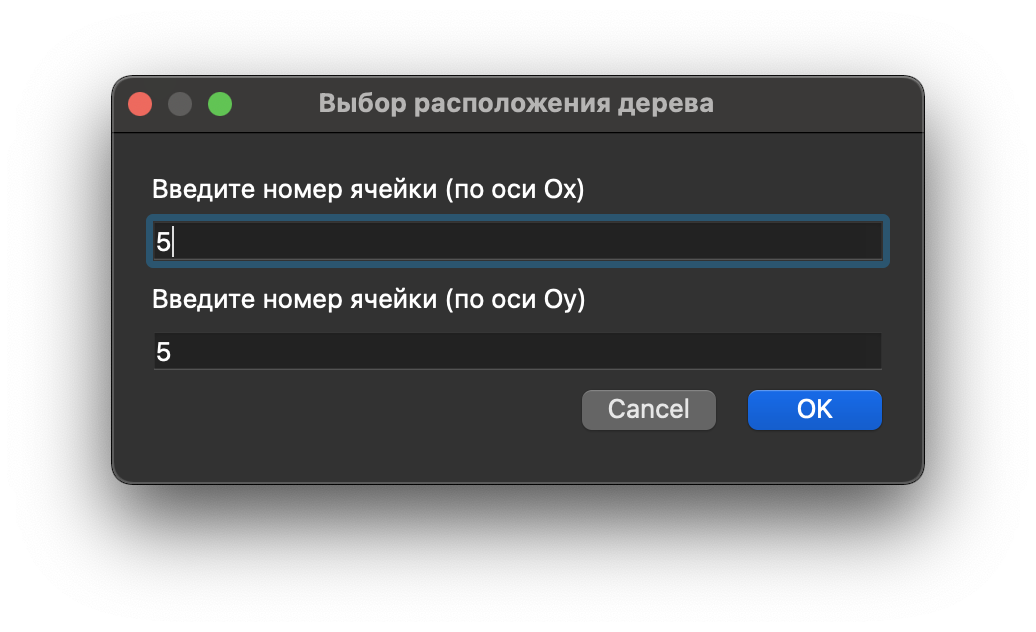
\includegraphics[scale=0.65]{img/tree.png}
	\caption{Интерфейс окна выбора распоожения дерева}
	\label{fig:tree}
\end{figure} 

\begin{figure}[h]
	\centering
	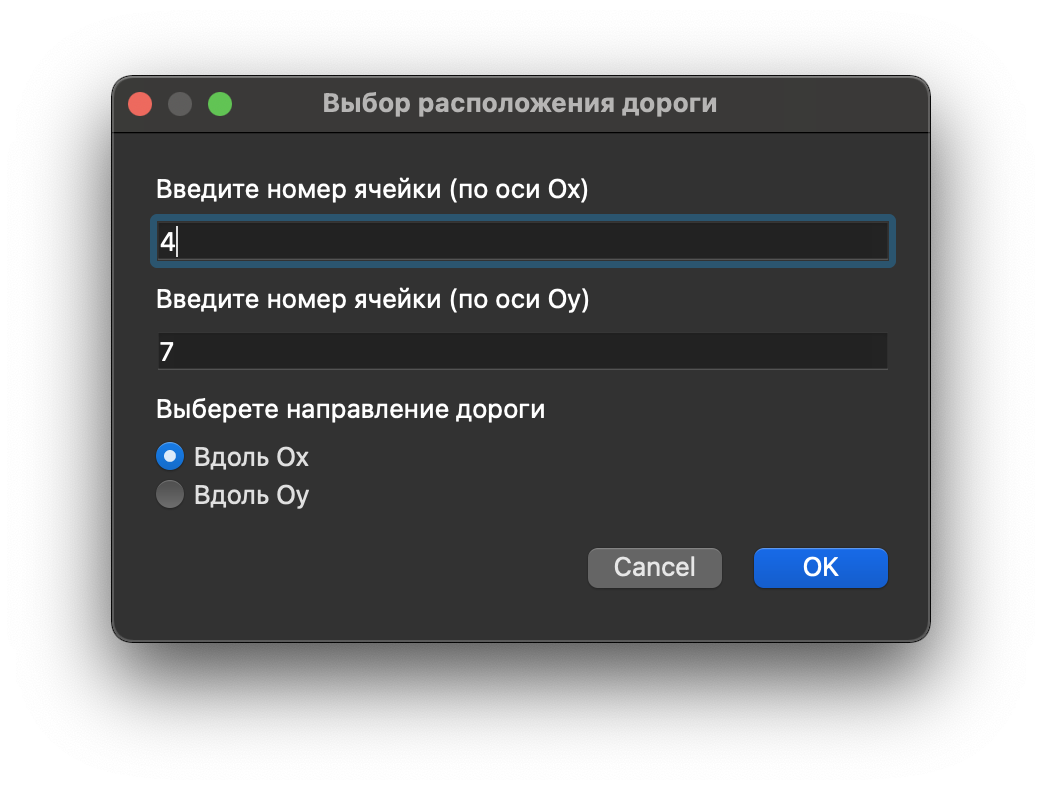
\includegraphics[scale=0.65]{img/road.png}
	\caption{Интерфейс окна выбора распоожения дороги}
	\label{fig:road}
\end{figure} 

\begin{figure}[h]
	\centering
	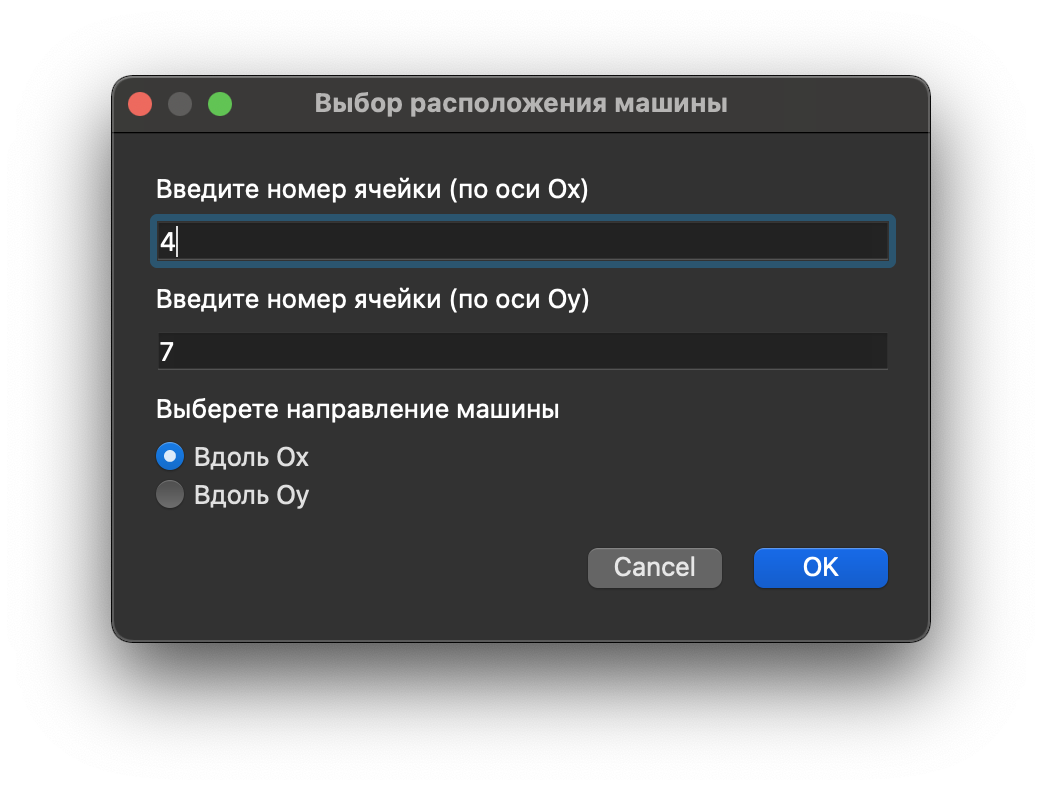
\includegraphics[scale=0.65]{img/car.png}
	\caption{Интерфейс окна выбора распоожения машины}
	\label{fig:car}
\end{figure} 

\begin{figure}[h]
	\centering
	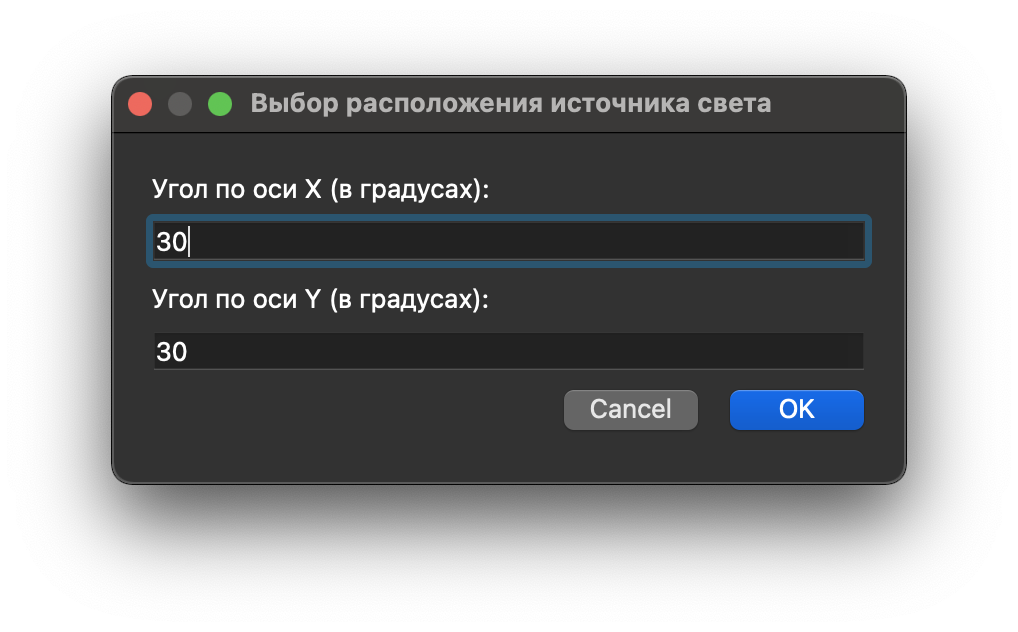
\includegraphics[scale=0.65]{img/illuminant.png}
	\caption{Интерфейс окна выбора распоожения источника света}
	\label{fig:illuminant}
\end{figure} 

\clearpage

На рисунках \ref{fig:change1} - \ref{fig:change2} изображены интерфейсы окон для перемещения  объетов по сетке сцены. 

\begin{figure}[h]
	\centering
	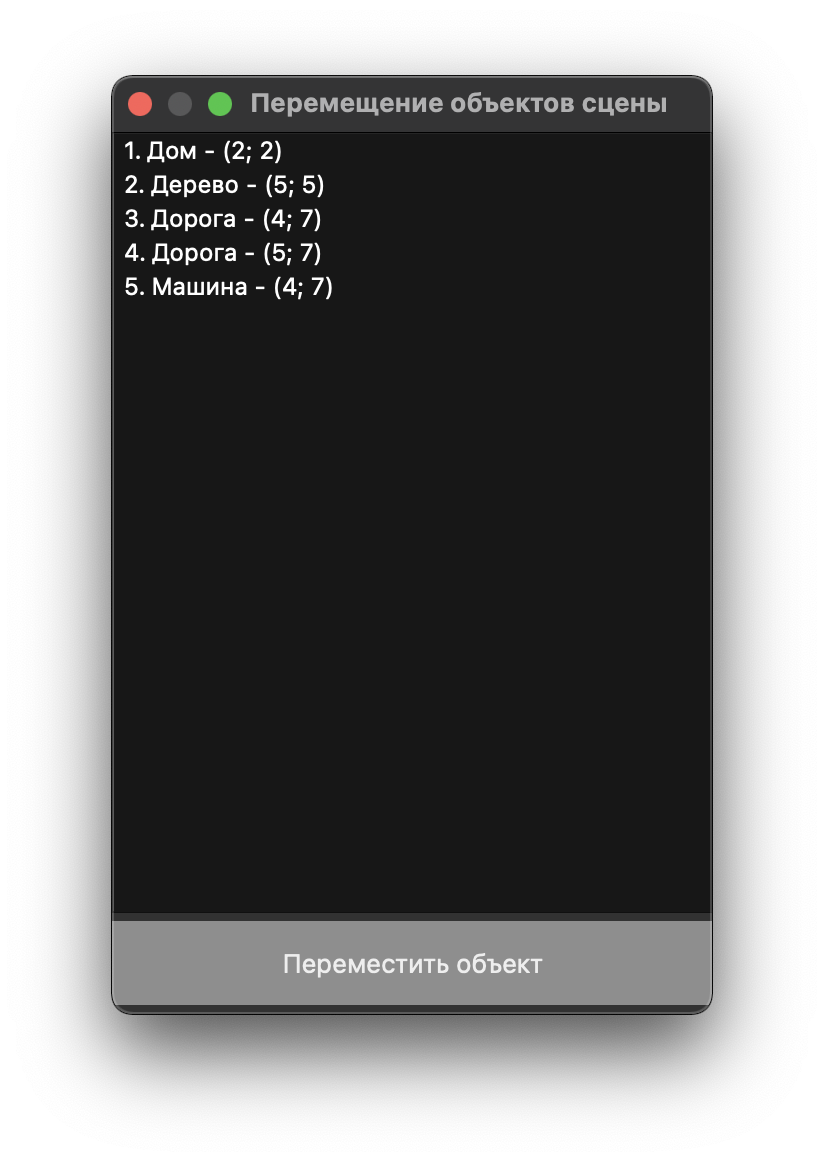
\includegraphics[scale=0.57]{img/change1.png}
	\caption{Интерфейс окна выбора перемещаемого объекта}
	\label{fig:change1}
\end{figure} 

\begin{figure}[h]
	\centering
	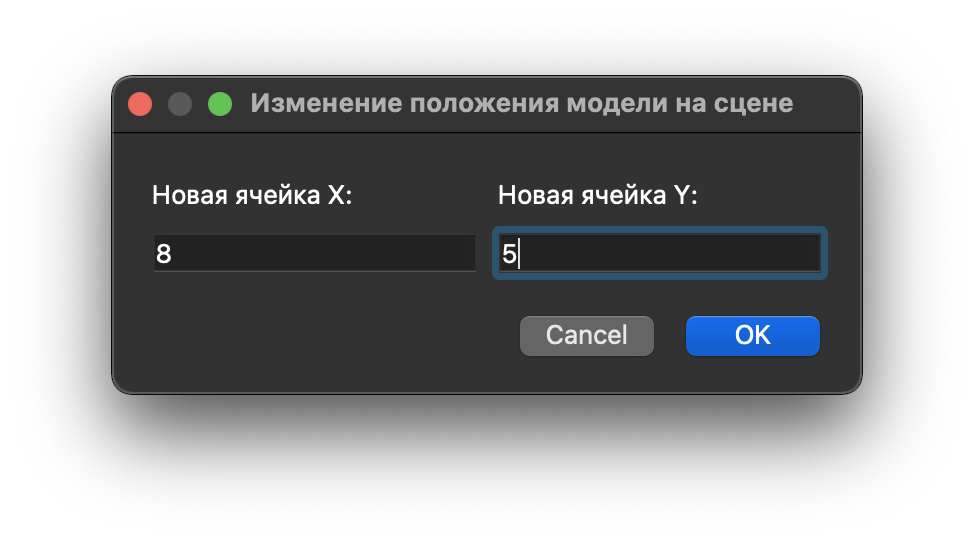
\includegraphics[scale=0.56]{img/change2.png}
	\caption{Интерфейс окна выбора нового расположения объекта}
	\label{fig:change2}
\end{figure} 

\clearpage

На рисунке \ref{fig:deletion} изображен интерфейс окна для удаления объетов со сцены. 

\begin{figure}[h]
	\centering
	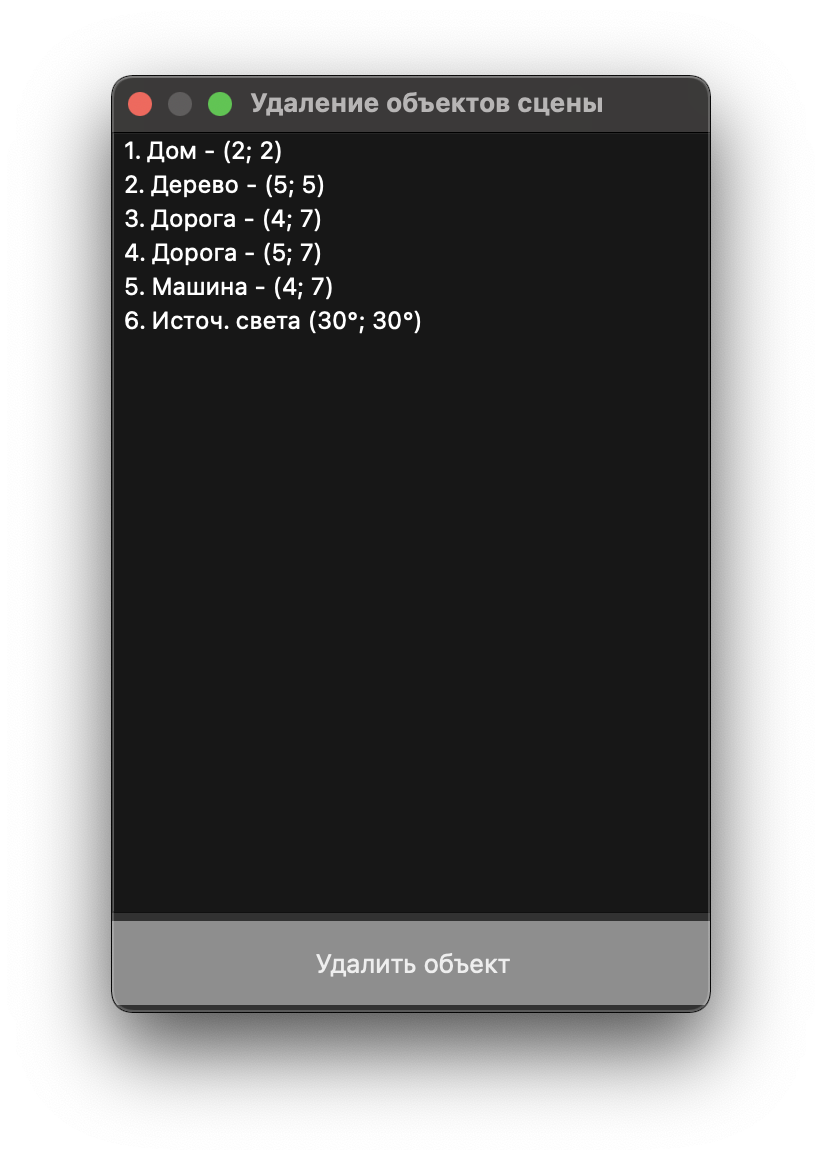
\includegraphics[scale=0.6]{img/deletion.png}
	\caption{Интерфейс окна выбора удаляемого объекта}
	\label{fig:deletion}
\end{figure} 

\section{Вывод}

В данном разделе были выбраны язык программирования и среда разработки, описаны поля реализуемых классов, сведения о модулях программы, а также интерфейс програмного обеспечения.

\chapter{Исследовательская часть}

В данном разделе будут приведены результаты работы программного обеспечения и проведен экмперимент с использованием библиотеки $OpenMP$.

\section{Результаты работы ПО}

На рисунке \ref{fig:example} приведен результат работы программы при наличии единственного источника света с заданными углами поворота в 30° по осям $X$ и $Y$.

\begin{figure}[h]
	\centering
	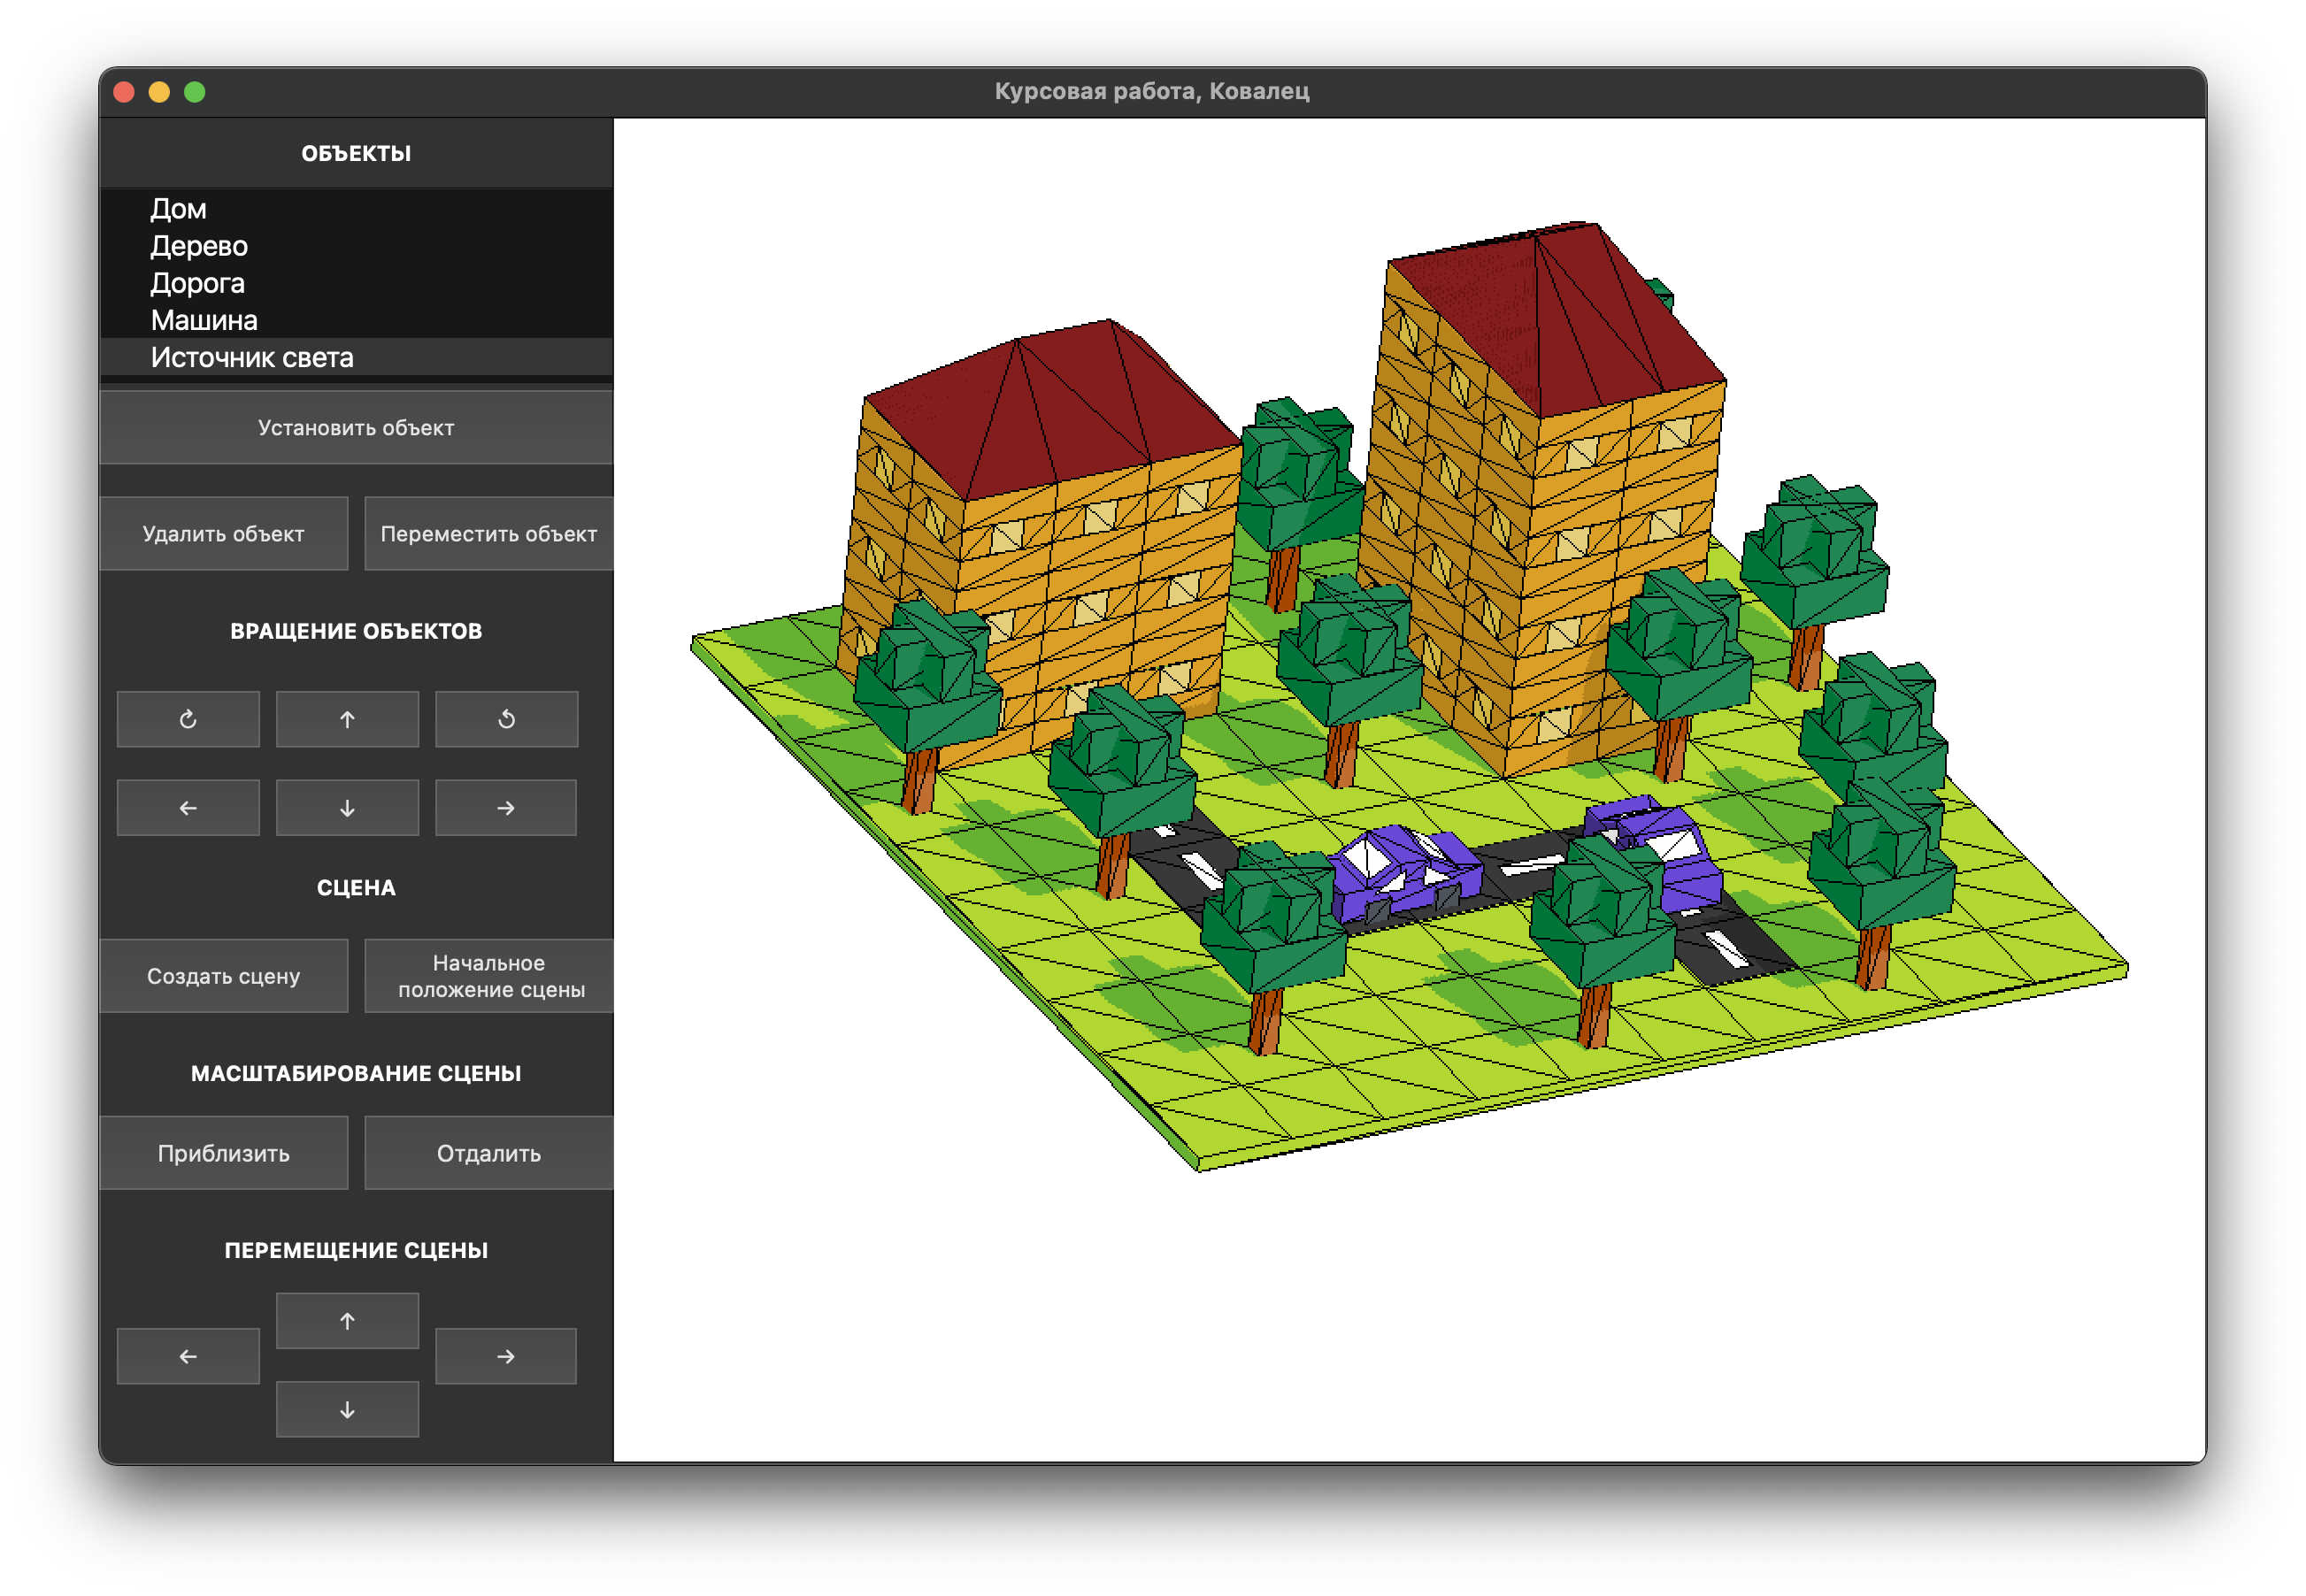
\includegraphics[scale=0.36]{img/example.png}
	\caption{Результат работы ПО с одним источником света}
	\label{fig:example}
\end{figure} 

\clearpage

На рисунке \ref{fig:example2} приведен результат работы программы при наличии двух рядом расположенных источников света с заданными углами поворота в 20\textdegree, \ 30\textdegree \ и 30\textdegree, \ 30\textdegree \ по осям $X$ и $Y$. В сравнении с рисунком \ref{fig:example} тени уменьшились.

\begin{figure}[h]
	\centering
	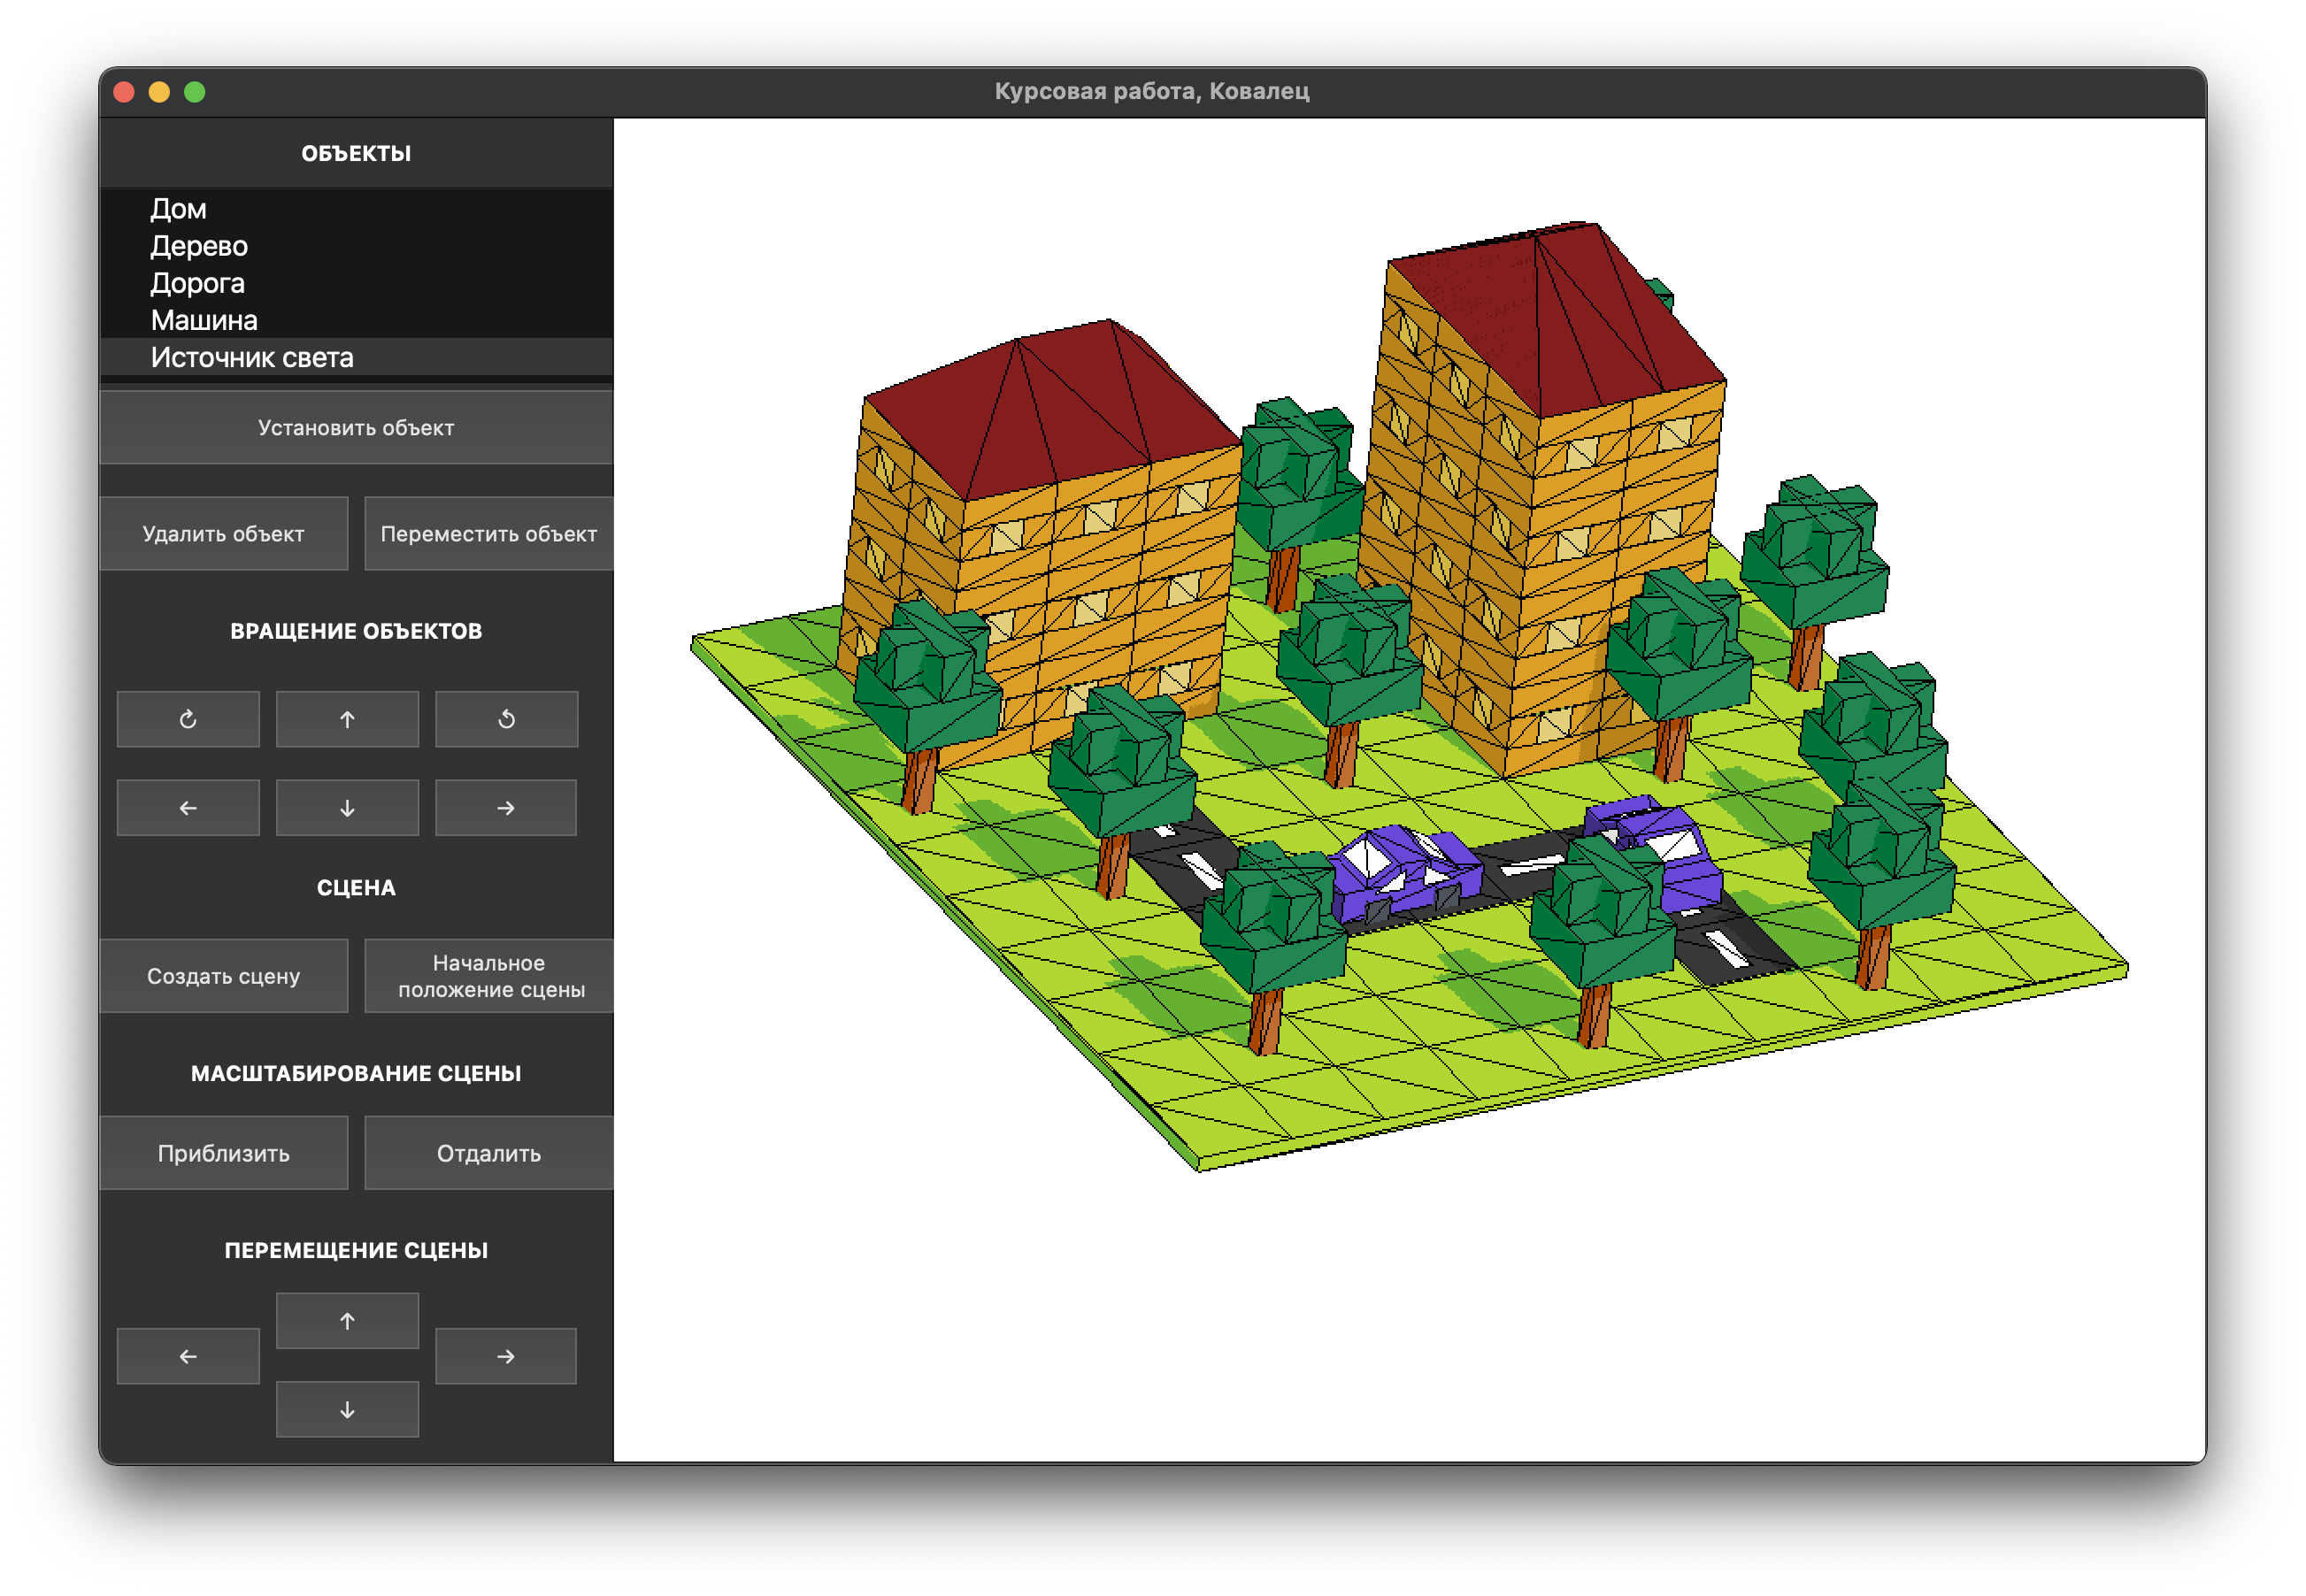
\includegraphics[scale=0.36]{img/example2.png}
	\caption{Результат работы ПО с двумя источниками света}
	\label{fig:example2}
\end{figure} 

\clearpage

На рисунке \ref{fig:example3} приведен результат работы программы при наличии единственного источника света с заданными углами поворота в 45° по осям $X$ и $Y$.

\begin{figure}[h]
	\centering
	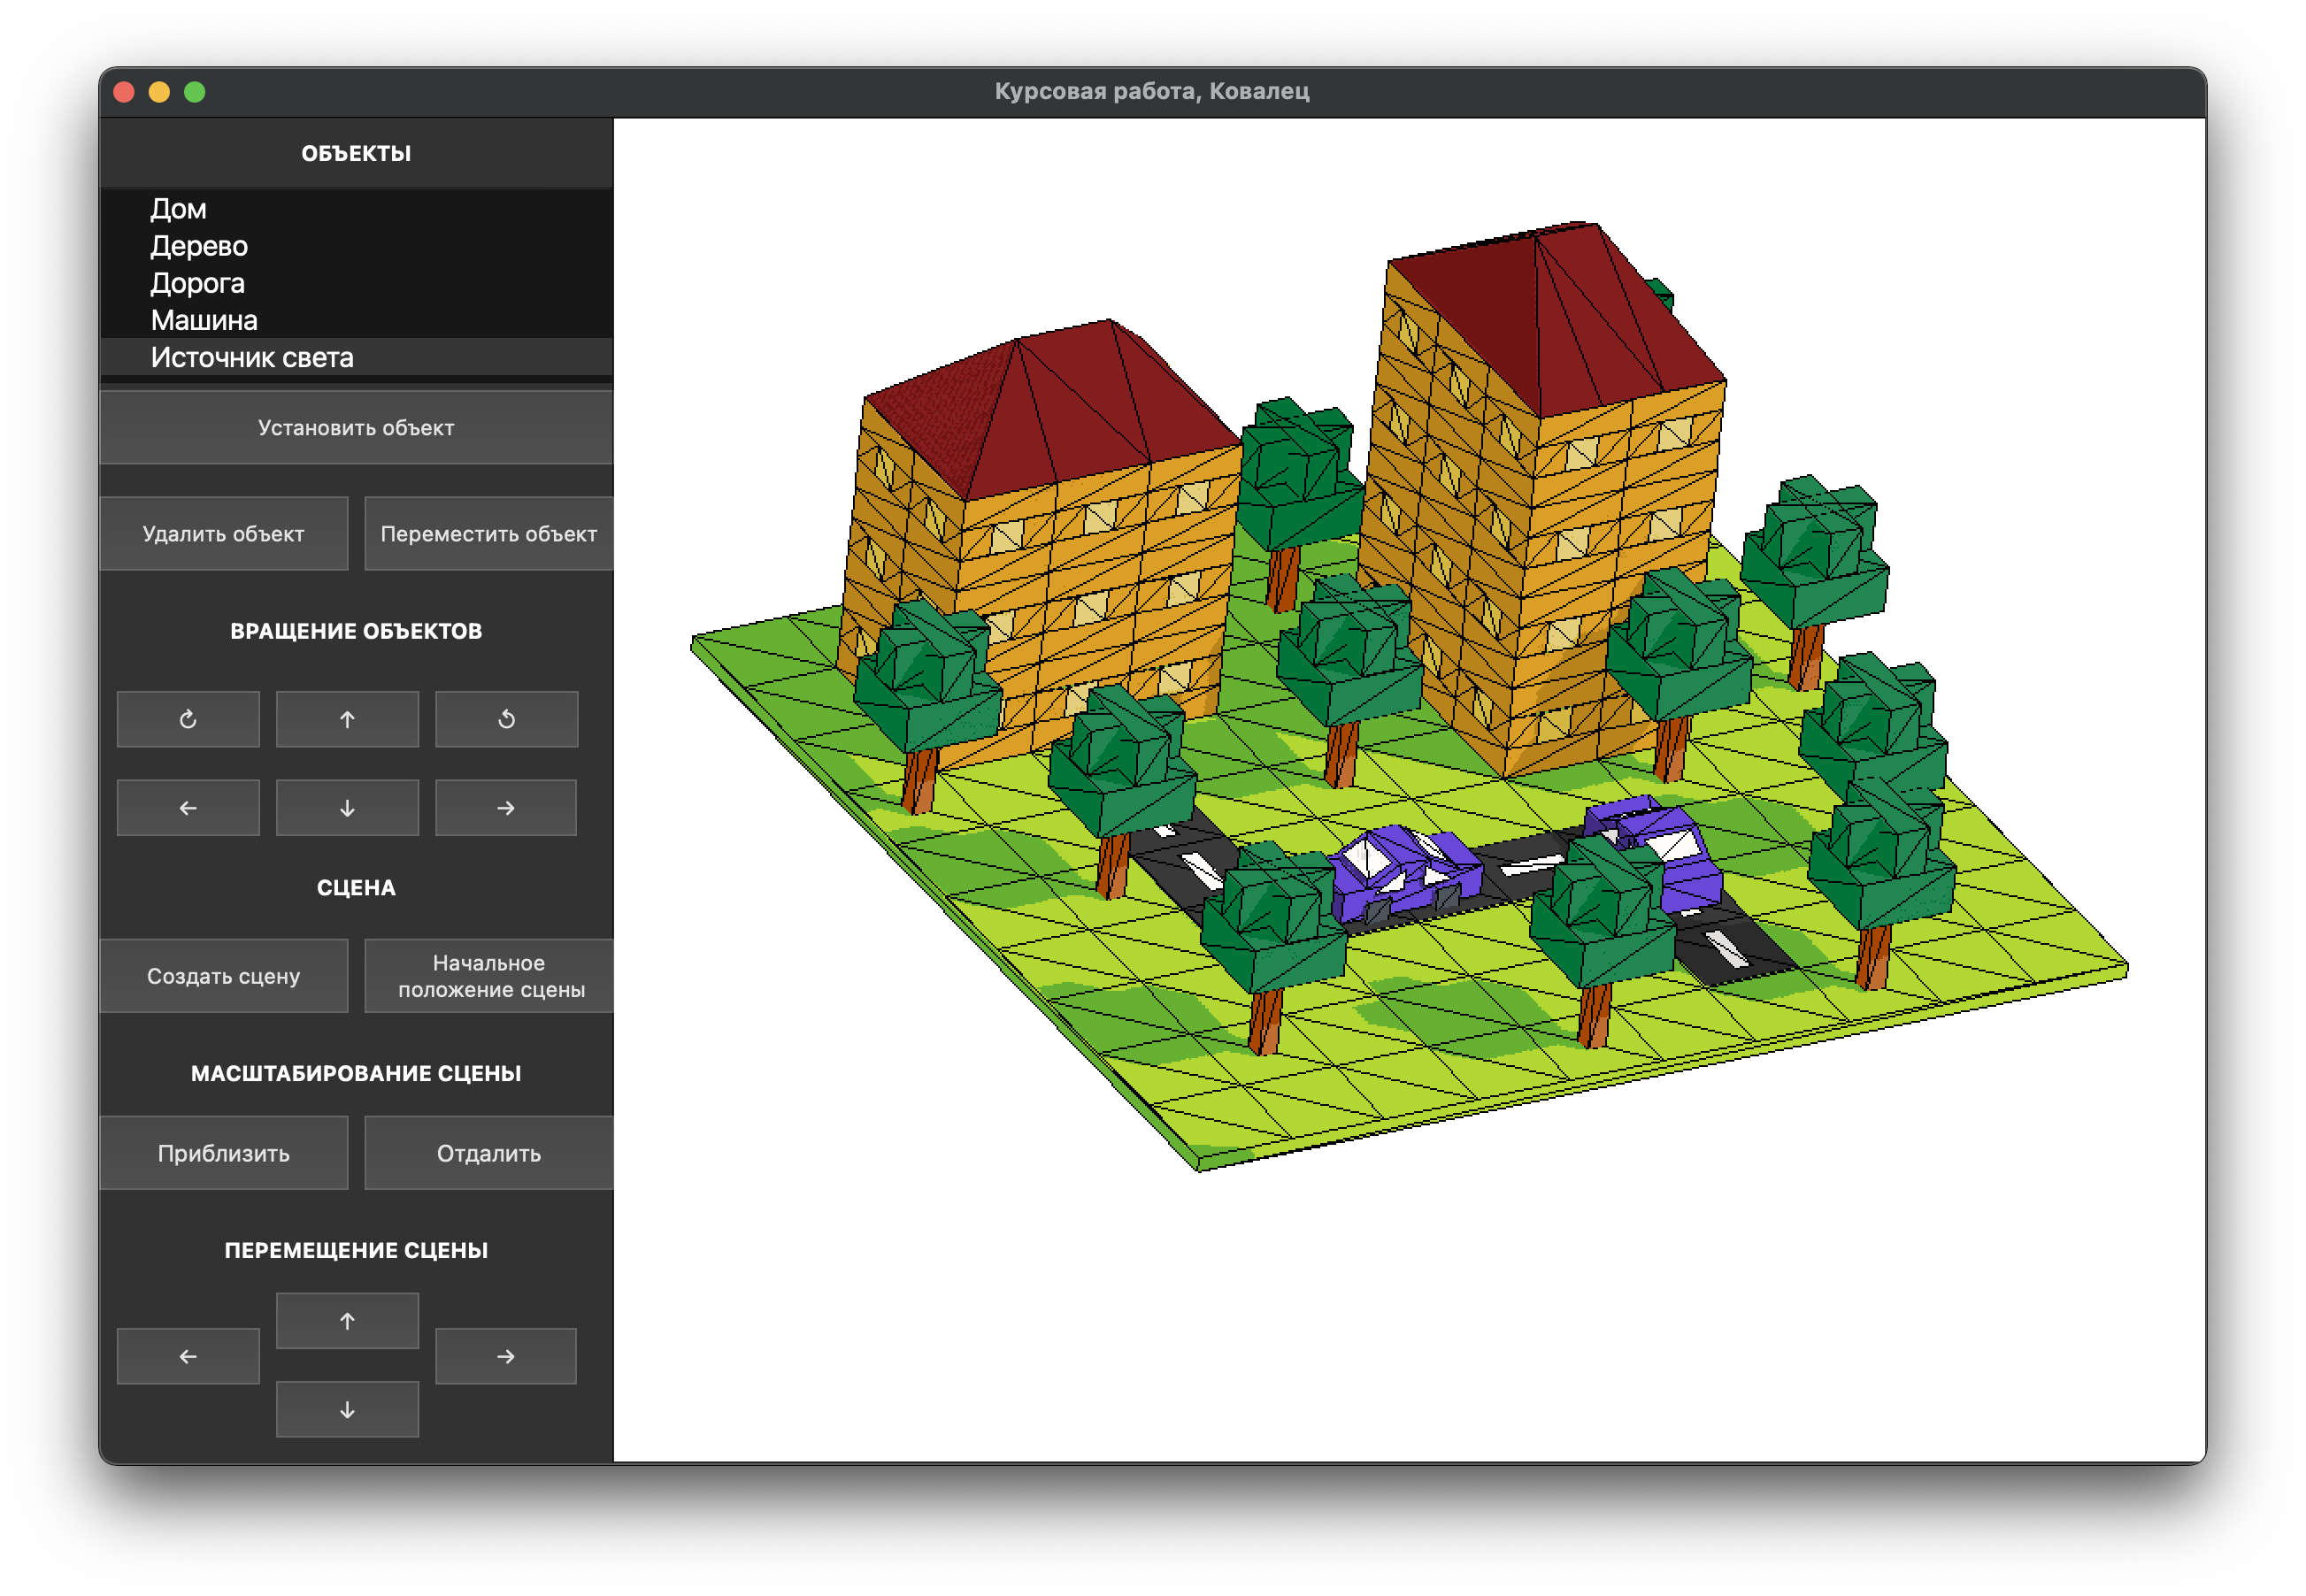
\includegraphics[scale=0.36]{img/example3.png}
	\caption{Результат работы ПО с измененным положением источника света}
	\label{fig:example3}
\end{figure} 

На рисунках \ref{fig:example4} - \ref{fig:example5} приведены результаты работы этой же программы, но с другого ракурса на сцену.

\begin{figure}[h]
	\centering
	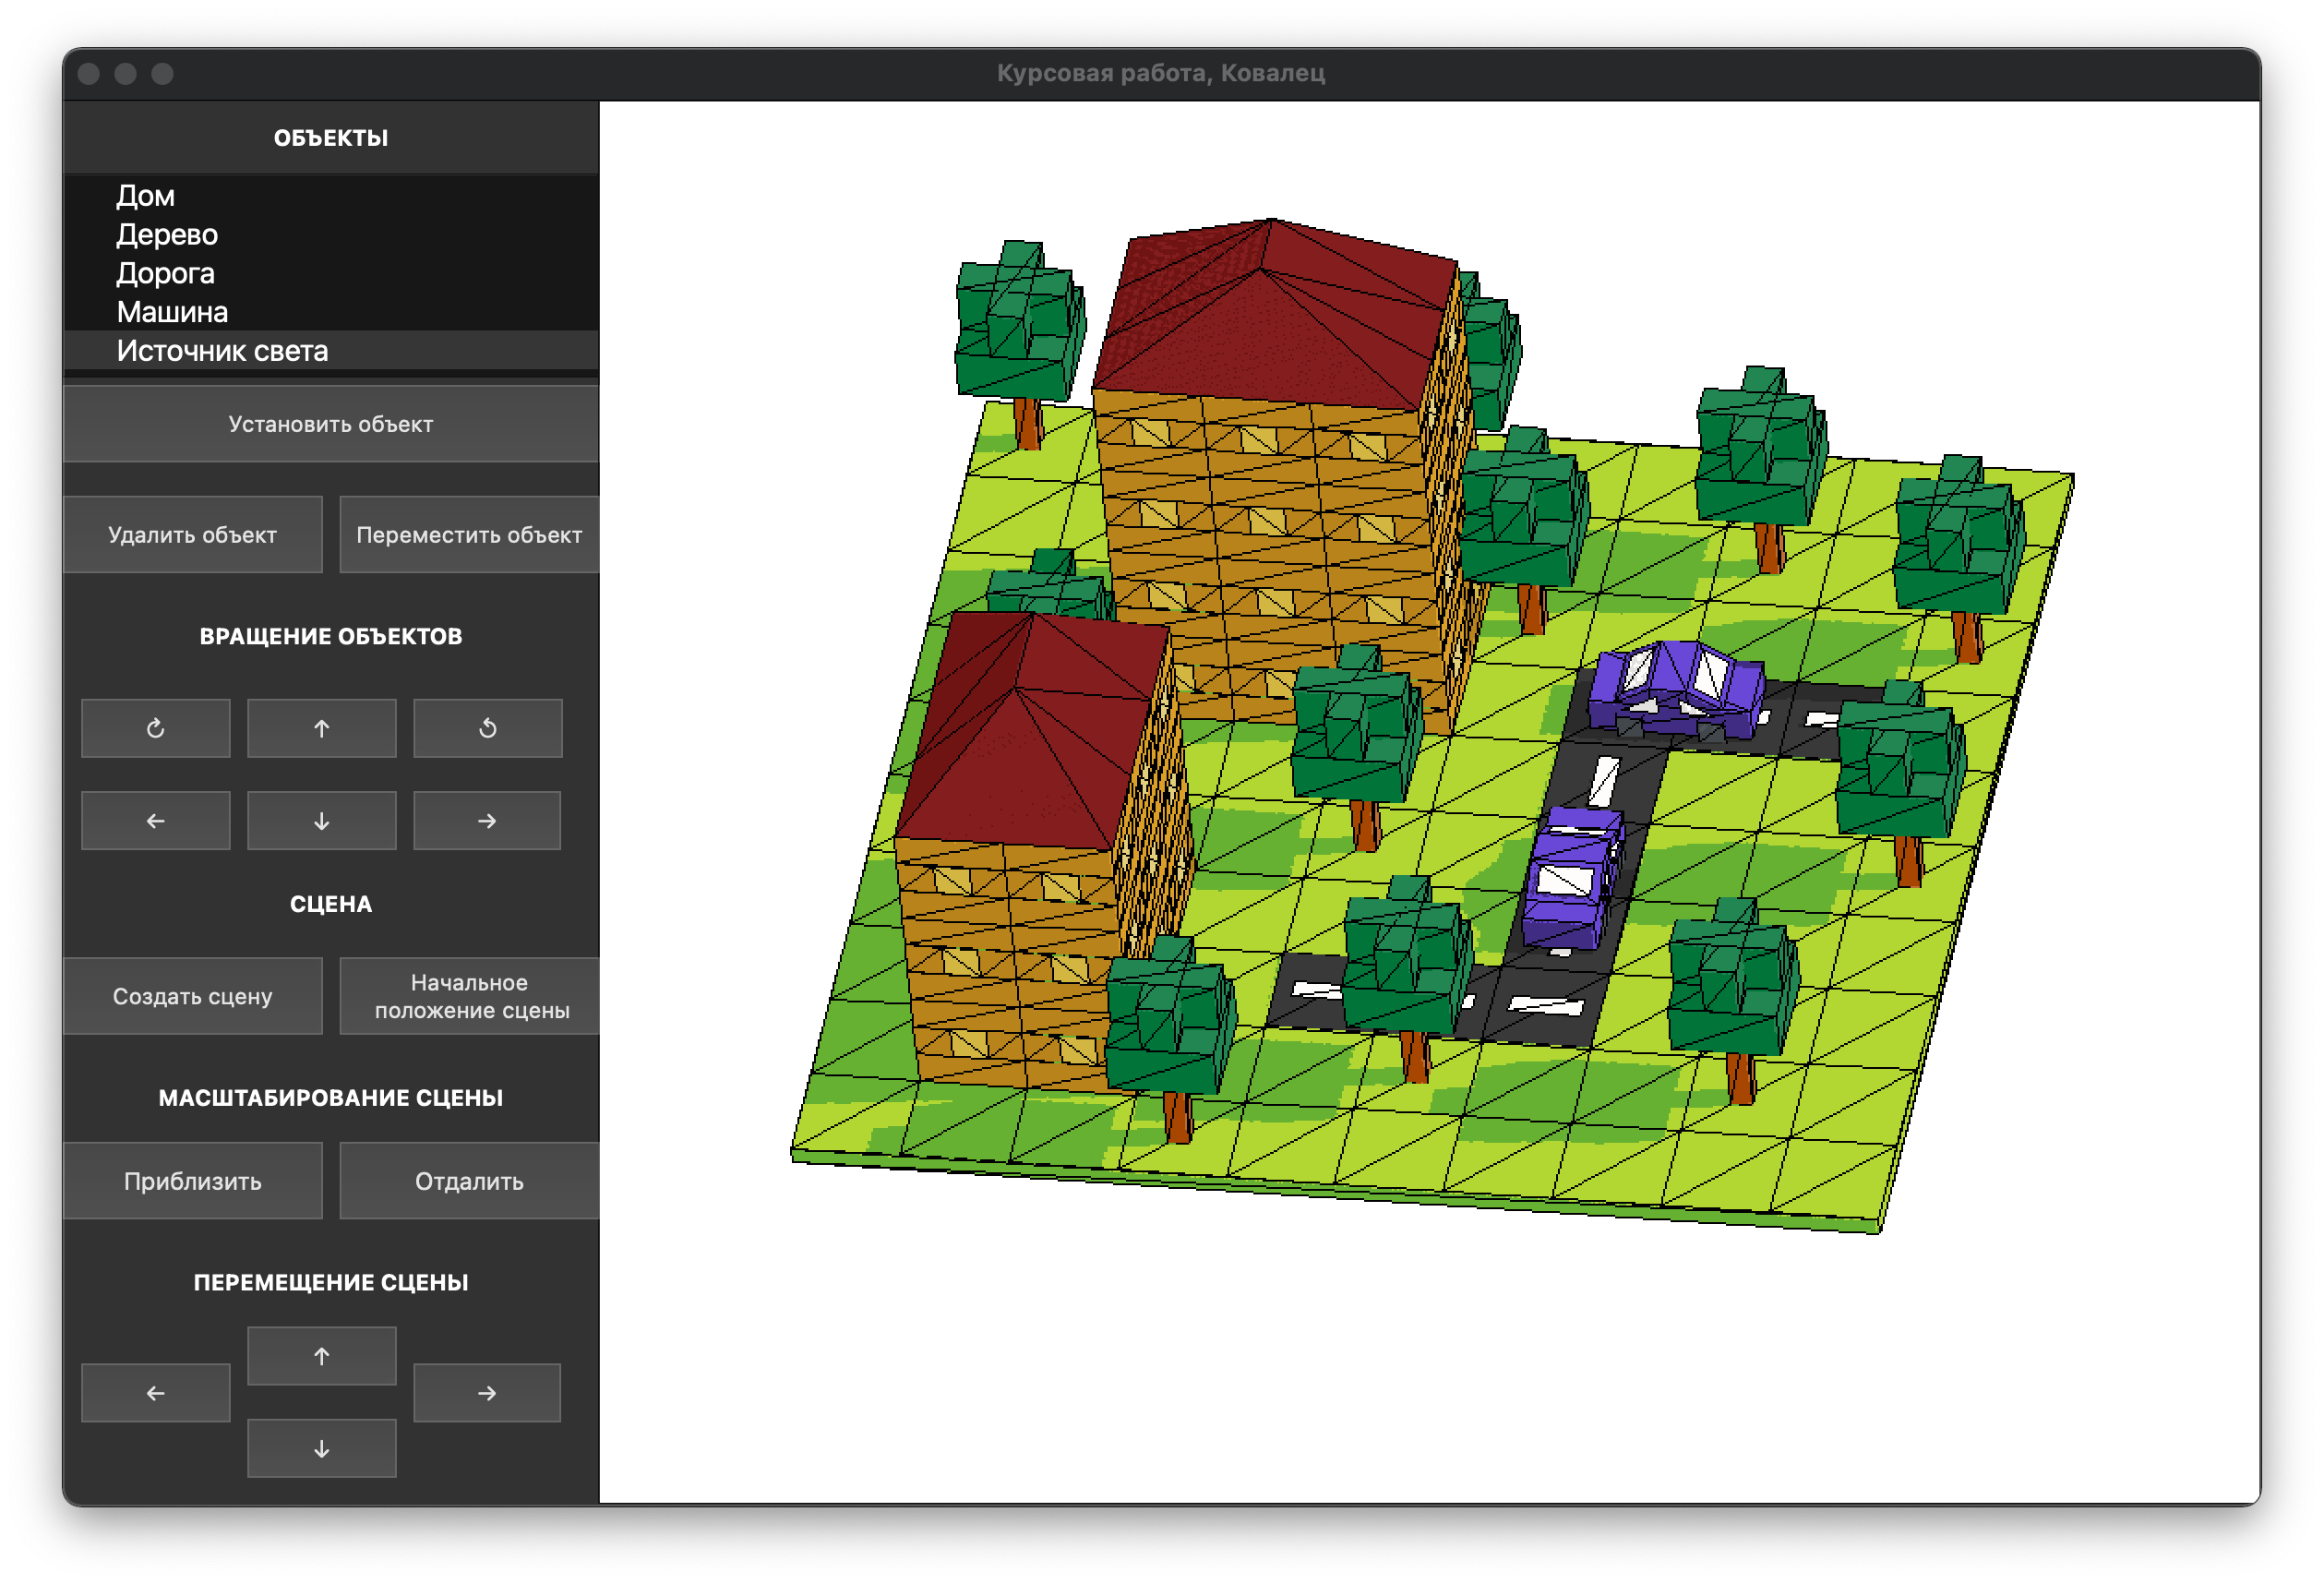
\includegraphics[scale=0.36]{img/example4.png}
	\caption{Результат работы ПО c другого ракурса}
	\label{fig:example4}
\end{figure} 

\begin{figure}[h]
	\centering
	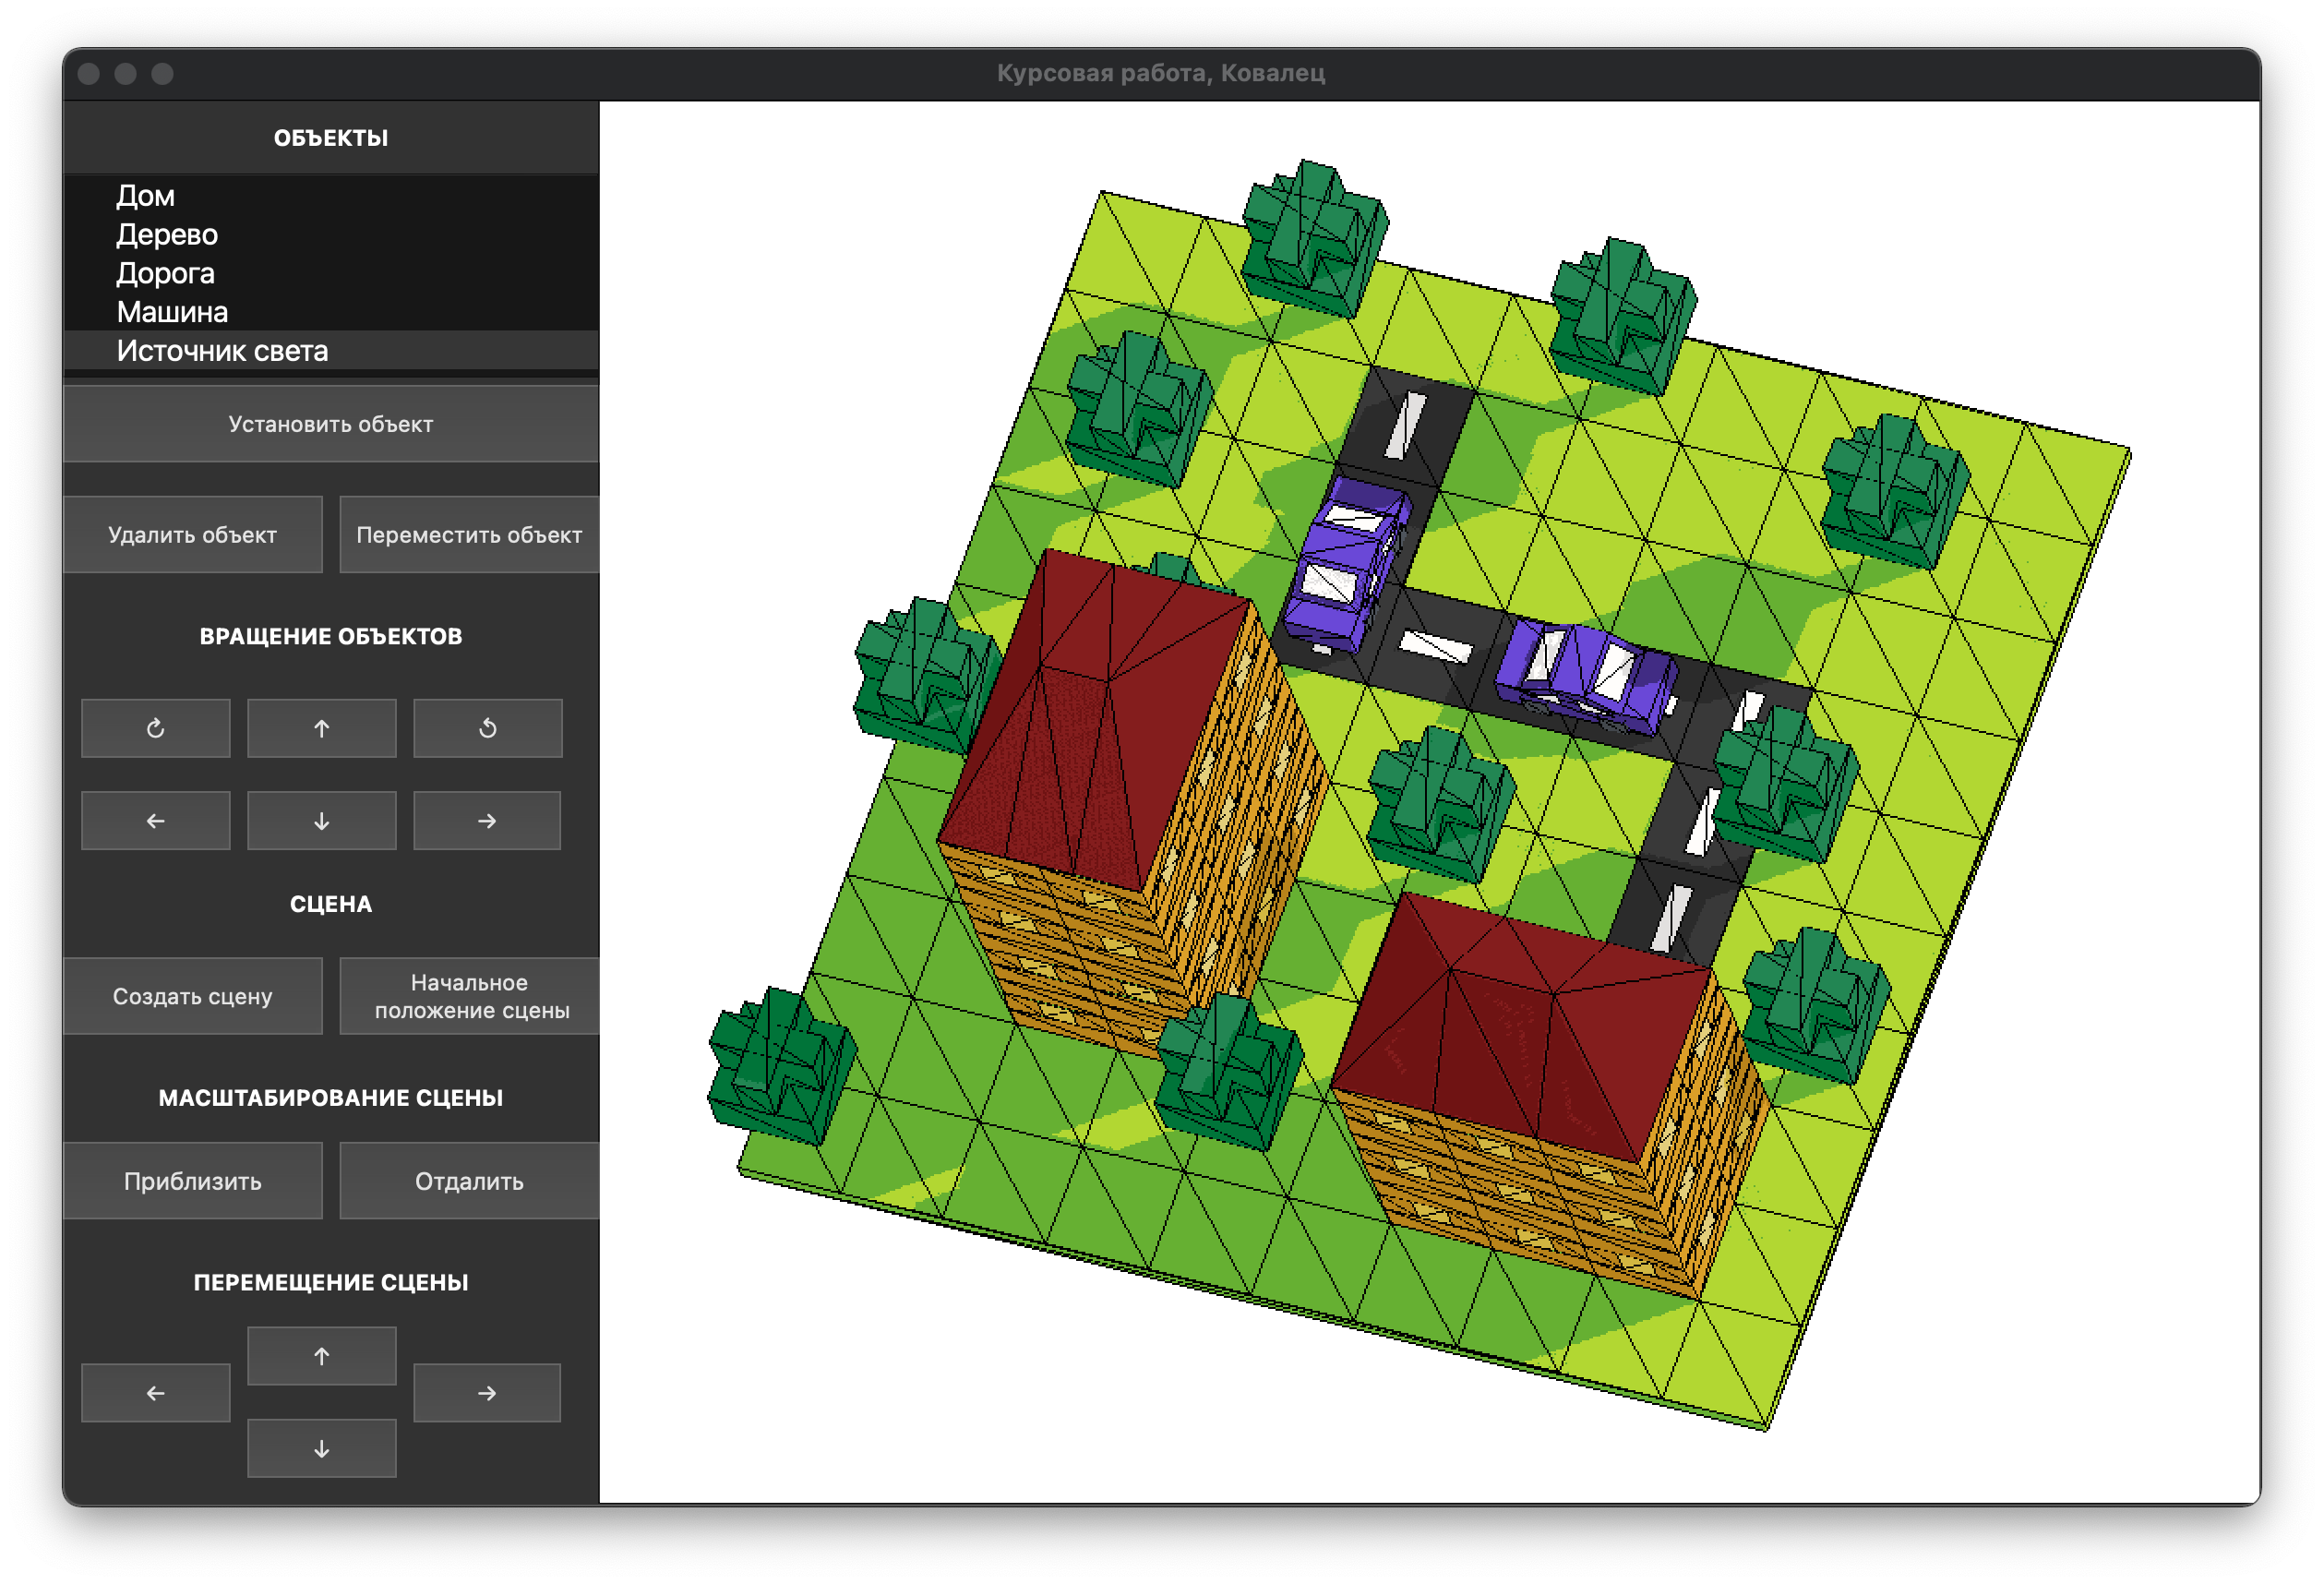
\includegraphics[scale=0.36]{img/example5.png}
	\caption{Результат работы ПО c другого ракурса}
	\label{fig:example5}
\end{figure} 

\clearpage

\section{Постановка эксперимента}

Для ускорения отрисовки сцены и объектов на ней было использовано распараллеливание циклов с помощью директив библиотеки $OpenMP$.

\subsection{Цель эксперимета}

Целью эксперимента является проведение сравнения скорости работы алгоритма z-буфера без использования и с использованием распараллеливания циклов при различных размерах сцены.

\subsection{Технические характеристики}

Технические характеристики устройства, на котором выполнялось тестирование представлены далее.

\begin{itemize}
    \item Операционная система: macOS 11.5.2.
    \item Память: 8 GiB.
    \item Процессор: 2,3 GHz 4-ядерный процессор Intel Core i5.
\end{itemize}

При тестировании ноутбук был включен в сеть электропитания. Во время тестирования ноутбук был нагружен только встроенными приложениями окружения, а также системой тестирования.

\subsection{Результаты эксперимента}

Результаты замеров времени работы z-буфера без использования и с использованием распараллеливания циклов при различных размерах сцены приведены в таблице \ref{tbl:table_2}. На рисунке 4.2 приведён график зависимости времени выполнения алгоритма z-буфера от размеров задаваемой сцены.

\begin{center}
\captionsetup{justification=raggedright,singlelinecheck=off}
\begin{longtable}[c]{|l|l|l|}
\caption{Результаты замеров времени работы z-буфера при различных размерах сцены\label{tbl:table_2}}
	\\ \hline
	\textbf{Размеры сцены} & \textbf{Время выполнения} &  \textbf{Время выполнения}
	\\ & \textbf{без использования} & \textbf{с использованием}
	\\ & \textbf{распараллеливания, мс} & \textbf{распараллеливания, мс}
	\\ \hline
	1x1 & 25 & 33
	\\ \hline
	10x10 & 152 & 92
	\\ \hline
	20x20 & 203 & 123
	\\ \hline
	30x30 & 227 & 163
	\\ \hline
	40x40 & 251 & 195
	\\ \hline
	50x50 & 296 & 242
	\\ \hline
\end{longtable}
\end{center}

\begin{figure}[h]
	\centering
	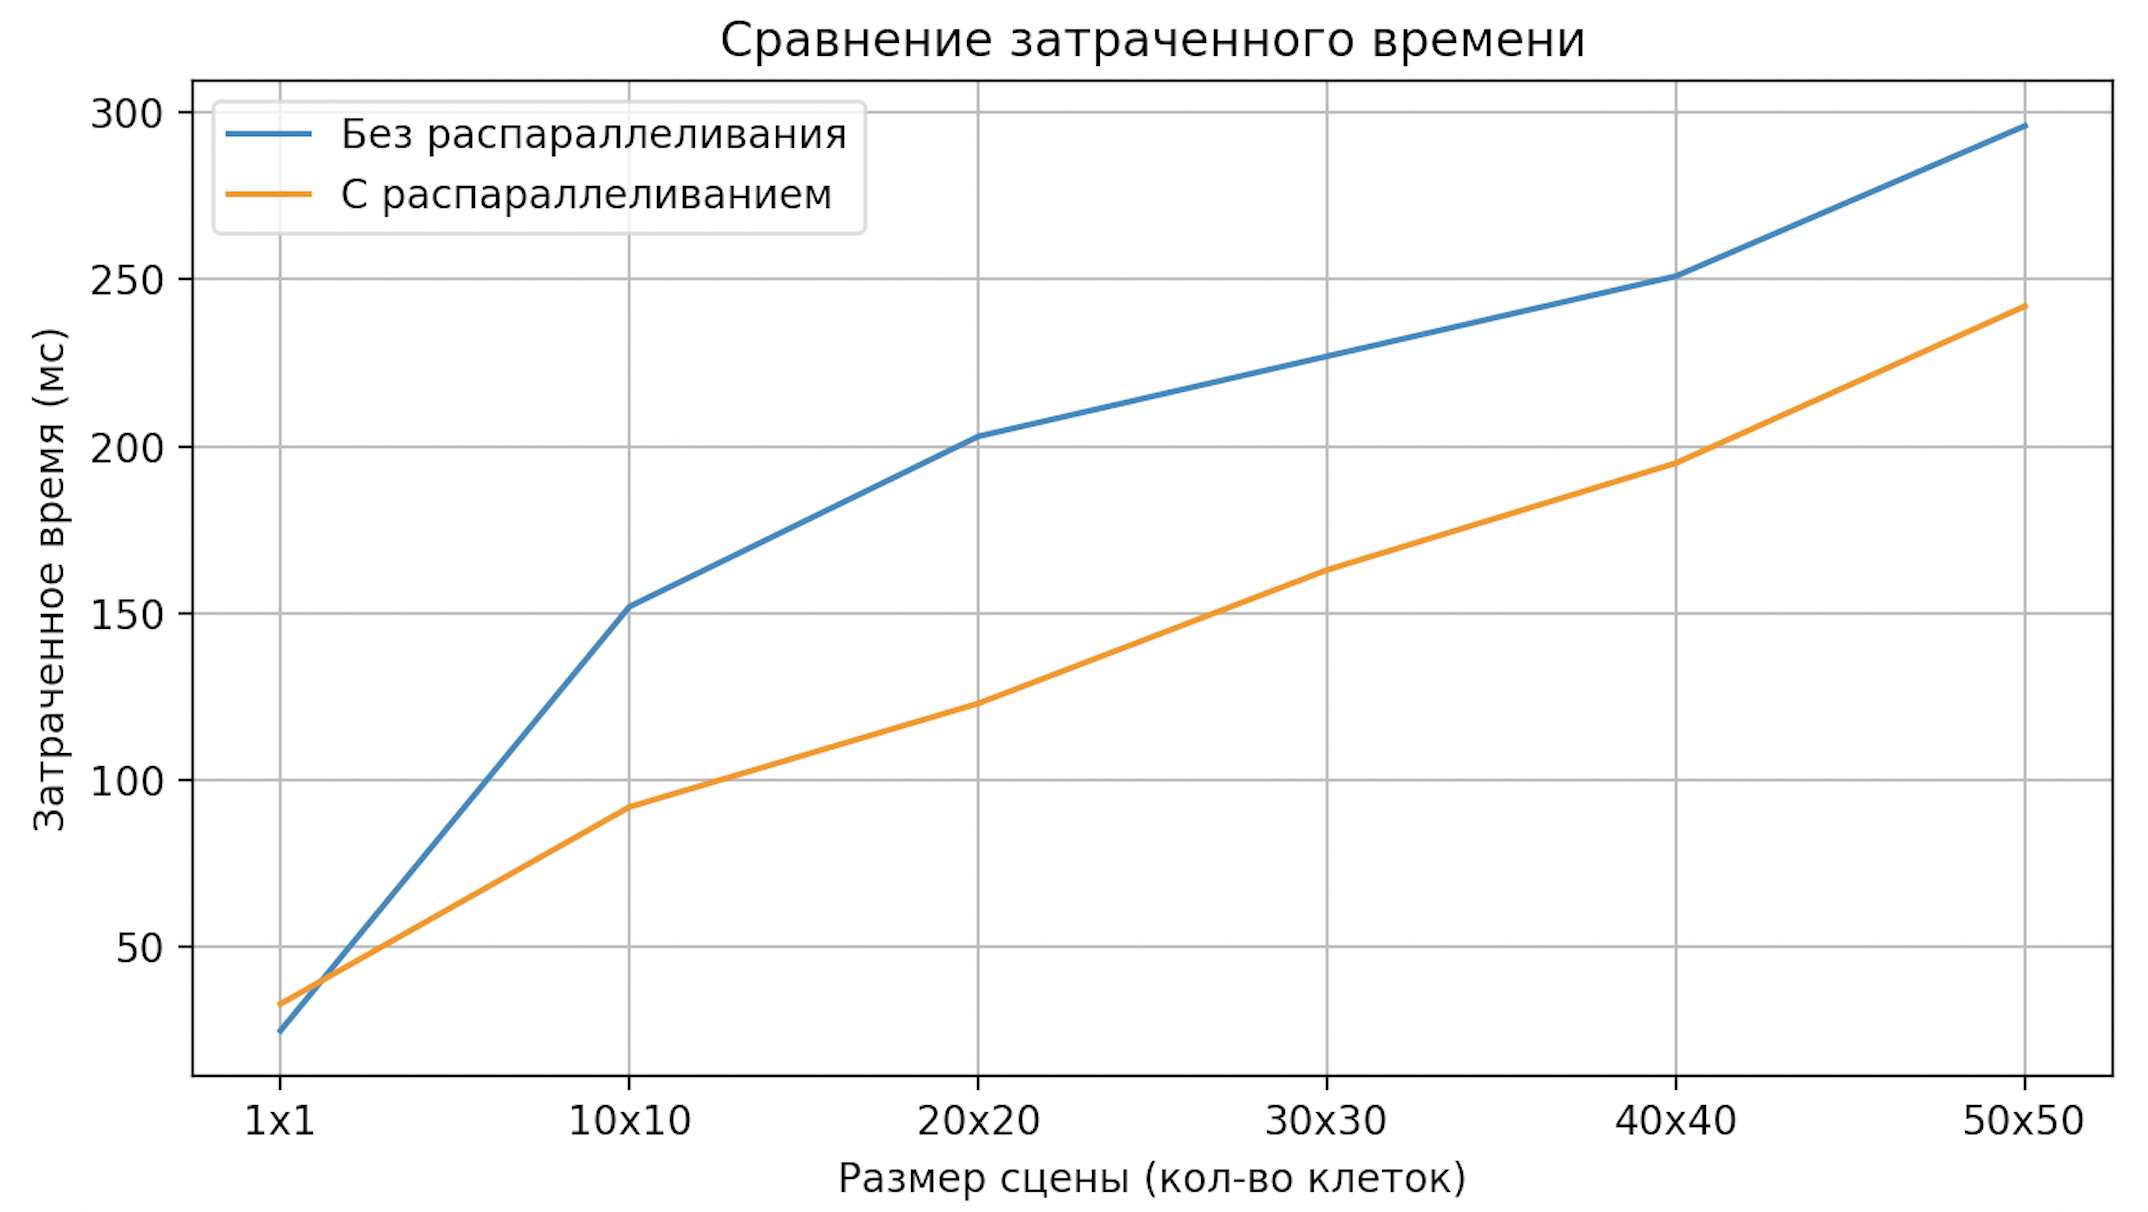
\includegraphics[scale=0.45]{img/time.png}
	\caption{График зависимости времени выполнения алгоритма z-буфера от размеров задаваемой сцены}
	\label{fig:time}
\end{figure} 

\clearpage

\section{Вывод}


В этом разделе были приведены результаты работы программного обеспечения и проведен экмперимент с использованием библиотеки $OpenMP$. Также были указаны характеристики машины, на которой происходило сравнение времени работы алгоритма z-буффера с использованием и без использования распараллеливания.

В результате эксперимента было установлено, что использование распараллеливания с помощью директив библиотеки $OpenMP$ помогло ускорить работу алгоритма z-буффера для всех рассмотренных размеров сцены, кроме сцены размером $1\times1$. На графике видно, что максимальная эффективность ускорения алгоритма z-буффера наблюдалась при построении сцен размерами $10\times10$ и $20\times20$ (в обоих случаях распараллеливание помогло ускорить работу алгоритма в 1.65 раз). Наименьшая эффективность (если не учитывать сцену размером $1\times1$) наблюдалась при построении сцены размером $50\times50$ (распараллеливание помогло ускорить работу алгоритма всего в 1.22 раза).


\chapter*{Заключение}
\addcontentsline{toc}{chapter}{Заключение}

Во время выполнения курсовой работы было реализовано программное обеспечение для решения задачи визуализации городского пространства. 

Были рассмотрены способы задания трехмерных моделей и выбрана поверхностная форма задания моделей. Также были рассмотрены алгоритмы удаления невидимых ребер (алгоритм, использующий z-буфер, алгоритм Робертса, алгоритм обратной трассировки лучей).

В качестве реализуемого был выбран алгоритм z-буфера, отвечающего двум требованиям: быстрая работа с множеством объектов сцены и преобладание скорости над точностью. Были рассмотрены алгоритмы построения теней. В качестве реализуемого был выбран алгоритм, использующий теневые карты, в работе которого будет использоваться z-буфер.

В ходе выполнения эксперимента в исследовательской части было установлено, что реализация алгоритма z-буфера с использованием директив, предоставляемых библиотекой $OpenMP$, позволяет ускорить реализованный алгоритм в лучшем случае в $1.65$ раза, что позволяет более быстро синтезировать изображение сцены.

Проделанная работа позволила лучше изучить как язык программирования С++, так и среду разработки Qt Creator.

Также в ходе выполнеия курсового проекта были выполнены следующие задачи:

\begin{itemize}
	\item описан список доступных к размещению на сцене моделей, а сами модели были  формализованы;
	\item выбраны существующие алгоритмы компьютерной графики для визуализации сцены и объектов на ней;
	\item выбран язык программирования и среда разработки;
	\item реализованы выбранные алгоритмы визуализации;
	\item реализовано программное обеспечения для визуализации и редактирования городского пространства.
\end{itemize}

Поставленная цель была достигнута.

\begin{thebibliography}{9}
	\bibitem{bib1}
	Демин А. Ю., Основы компьютерной графики [Электронный ресурс] // Томс, Томский политехнический университет. 2011. URL: \url{https://portal.tpu.ru/SHARED/j/JBOLOTOVA/academic/ComputerGraphics/CGStudyBook.pdf}.
	\bibitem{bib2}
	Набережнов Г. М., Максимов, Н. Н. Трехмерное моделирование полигональными сетками [Электронный ресурс] // Казань, Казанский государственный технический университет им. А.Н.Туполева. 2008. URL: \url{https://studfile.net/preview/7335496/}.
	\bibitem{bib3}
	Польский С. В., Компьютерная графика [Электронный ресурс] // Москва, Московский государственный университет леса. 2008. URL: \url{https://mf.bmstu.ru/info/faculty/kf/caf/k3/subjects/Computer_graphics/materials/CG_RGR.pdf}.
	\bibitem{bib4}
	Селянкин В. В., Алгоритмы трехмерной графики [Электронный ресурс] // Таганрог, Южный федеральный университет. 2007. URL: \url{http://ntb.tgn.sfedu.ru/UML/UML_4112.pdf}.
	\bibitem{bib5}
	Rogers D., Adams J., Matematical Elements for Computer Graphics [Электронный ресурс] // Аннаполис, United States Naval Academy. 1989. URL: \url{https://itslearningakarmazyan.files.wordpress.com/2015/08/rodzhers_adams.pdf}.
	\bibitem{bib6} Eck D., Introduction to Computer Graphics [Электронный ресурс] // Нью-Йорк, Hobart and William Smith Colleges. 2021. URL: \url{https://math.hws.edu/eck/cs424/downloads/graphicsbook-linked.pdf}.
	\bibitem{bib7}
	Programming Languages -- C++ [Электронный ресурс] // 2020. URL: \url{https://isocpp.org/files/papers/N4860.pdf}.
	\bibitem{bib8}
	Qt Documentation [Электронный ресурс] // URL: \url{https://doc.qt.io/qt-6/}.
	\bibitem{bib9}
	OpenMP Specifications [Электронный ресурс] // URL: \url{https://www.openmp.org/specifications/}.
\end{thebibliography}

\addcontentsline{toc}{chapter}{Список литературы}

\end{document}
